%%%%%%%%%%%%%%%%%%%%%%%%%%%%%%%%%%%%%%%%%%%%%%%%%%%%%%%%%%%%%%%
%% OXFORD THESIS TEMPLATE

% Use this template to produce a standard thesis that meets the Oxford University requirements for DPhil submission
%
% Originally by Keith A. Gillow (gillow@maths.ox.ac.uk), 1997
% Modified by Sam Evans (sam@samuelevansresearch.org), 2007
% Modified by John McManigle (john@oxfordechoes.com), 2015
% Modified by Ulrik Lyngs (ulrik.lyngs@cs.ox.ac.uk), 2018-, for use with R Markdown
%
% Ulrik Lyngs, 25 Nov 2018: Following John McManigle, broad permissions are granted to use, modify, and distribute this software
% as specified in the MIT License included in this distribution's LICENSE file.
%
% John commented this file extensively, so read through to see how to use the various options.  Remember that in LaTeX,
% any line starting with a % is NOT executed.

%%%%% PAGE LAYOUT
% The most common choices should be below.  You can also do other things, like replace "a4paper" with "letterpaper", etc.

% 'twoside' formats for two-sided binding (ie left and right pages have mirror margins; blank pages inserted where needed):
%\documentclass[a4paper,twoside]{templates/ociamthesis}
% Specifying nothing formats for one-sided binding (ie left margin > right margin; no extra blank pages):
%\documentclass[a4paper]{ociamthesis}
% 'nobind' formats for PDF output (ie equal margins, no extra blank pages):
%\documentclass[a4paper,nobind]{templates/ociamthesis}

% As you can see from the line below, oxforddown uses the a4paper size, 
% and passes in the binding option from the YAML header in index.Rmd:
\documentclass[a4paper, nobind]{templates/ociamthesis}


%%%%% ADDING LATEX PACKAGES
% add hyperref package with options from YAML %
\usepackage[pdfpagelabels]{hyperref}
% handle long urls
\usepackage{xurl}
% change the default coloring of links to something sensible
\usepackage{xcolor}

\definecolor{mylinkcolor}{RGB}{0,0,139}
\definecolor{myurlcolor}{RGB}{0,0,139}
\definecolor{mycitecolor}{RGB}{0,33,71}

\hypersetup{
  hidelinks,
  colorlinks,
  linktocpage=true,
  linkcolor=mylinkcolor,
  urlcolor=myurlcolor,
  citecolor=mycitecolor
}


% add float package to allow manual control of figure positioning %
\usepackage{float}

% enable strikethrough
\usepackage[normalem]{ulem}

% use soul package for correction highlighting
\usepackage{color, soulutf8}
\definecolor{correctioncolor}{HTML}{CCCCFF}
\sethlcolor{correctioncolor}
\newcommand{\ctext}[3][RGB]{%
  \begingroup
  \definecolor{hlcolor}{#1}{#2}\sethlcolor{hlcolor}%
  \hl{#3}%
  \endgroup
}
% stop soul from freaking out when it sees citation commands
\soulregister\ref7
\soulregister\cite7
\soulregister\citet7
\soulregister\autocite7
\soulregister\textcite7
\soulregister\pageref7

%%%%% FIXING / ADDING THINGS THAT'S SPECIAL TO R MARKDOWN'S USE OF LATEX TEMPLATES
% pandoc puts lists in 'tightlist' command when no space between bullet points in Rmd file,
% so we add this command to the template
\providecommand{\tightlist}{%
  \setlength{\itemsep}{0pt}\setlength{\parskip}{0pt}}
 
% allow us to include code blocks in shaded environments
\usepackage{color}
\usepackage{fancyvrb}
\newcommand{\VerbBar}{|}
\newcommand{\VERB}{\Verb[commandchars=\\\{\}]}
\DefineVerbatimEnvironment{Highlighting}{Verbatim}{commandchars=\\\{\}}
% Add ',fontsize=\small' for more characters per line
\usepackage{framed}
\definecolor{shadecolor}{RGB}{248,248,248}
\newenvironment{Shaded}{\begin{snugshade}}{\end{snugshade}}
\newcommand{\AlertTok}[1]{\textcolor[rgb]{0.94,0.16,0.16}{#1}}
\newcommand{\AnnotationTok}[1]{\textcolor[rgb]{0.56,0.35,0.01}{\textbf{\textit{#1}}}}
\newcommand{\AttributeTok}[1]{\textcolor[rgb]{0.13,0.29,0.53}{#1}}
\newcommand{\BaseNTok}[1]{\textcolor[rgb]{0.00,0.00,0.81}{#1}}
\newcommand{\BuiltInTok}[1]{#1}
\newcommand{\CharTok}[1]{\textcolor[rgb]{0.31,0.60,0.02}{#1}}
\newcommand{\CommentTok}[1]{\textcolor[rgb]{0.56,0.35,0.01}{\textit{#1}}}
\newcommand{\CommentVarTok}[1]{\textcolor[rgb]{0.56,0.35,0.01}{\textbf{\textit{#1}}}}
\newcommand{\ConstantTok}[1]{\textcolor[rgb]{0.56,0.35,0.01}{#1}}
\newcommand{\ControlFlowTok}[1]{\textcolor[rgb]{0.13,0.29,0.53}{\textbf{#1}}}
\newcommand{\DataTypeTok}[1]{\textcolor[rgb]{0.13,0.29,0.53}{#1}}
\newcommand{\DecValTok}[1]{\textcolor[rgb]{0.00,0.00,0.81}{#1}}
\newcommand{\DocumentationTok}[1]{\textcolor[rgb]{0.56,0.35,0.01}{\textbf{\textit{#1}}}}
\newcommand{\ErrorTok}[1]{\textcolor[rgb]{0.64,0.00,0.00}{\textbf{#1}}}
\newcommand{\ExtensionTok}[1]{#1}
\newcommand{\FloatTok}[1]{\textcolor[rgb]{0.00,0.00,0.81}{#1}}
\newcommand{\FunctionTok}[1]{\textcolor[rgb]{0.13,0.29,0.53}{\textbf{#1}}}
\newcommand{\ImportTok}[1]{#1}
\newcommand{\InformationTok}[1]{\textcolor[rgb]{0.56,0.35,0.01}{\textbf{\textit{#1}}}}
\newcommand{\KeywordTok}[1]{\textcolor[rgb]{0.13,0.29,0.53}{\textbf{#1}}}
\newcommand{\NormalTok}[1]{#1}
\newcommand{\OperatorTok}[1]{\textcolor[rgb]{0.81,0.36,0.00}{\textbf{#1}}}
\newcommand{\OtherTok}[1]{\textcolor[rgb]{0.56,0.35,0.01}{#1}}
\newcommand{\PreprocessorTok}[1]{\textcolor[rgb]{0.56,0.35,0.01}{\textit{#1}}}
\newcommand{\RegionMarkerTok}[1]{#1}
\newcommand{\SpecialCharTok}[1]{\textcolor[rgb]{0.81,0.36,0.00}{\textbf{#1}}}
\newcommand{\SpecialStringTok}[1]{\textcolor[rgb]{0.31,0.60,0.02}{#1}}
\newcommand{\StringTok}[1]{\textcolor[rgb]{0.31,0.60,0.02}{#1}}
\newcommand{\VariableTok}[1]{\textcolor[rgb]{0.00,0.00,0.00}{#1}}
\newcommand{\VerbatimStringTok}[1]{\textcolor[rgb]{0.31,0.60,0.02}{#1}}
\newcommand{\WarningTok}[1]{\textcolor[rgb]{0.56,0.35,0.01}{\textbf{\textit{#1}}}}

% set white space before and after code blocks


\renewenvironment{Shaded}
{
  \vspace{10pt}%
  \begin{snugshade}%
}{%
  \end{snugshade}%
  \vspace{8pt}%
}

% User-included things with header_includes or in_header will appear here
% kableExtra packages will appear here if you use library(kableExtra)
\usepackage{booktabs}
\usepackage{longtable}
\usepackage{array}
\usepackage{multirow}
\usepackage{wrapfig}
\usepackage{float}
\usepackage{colortbl}
\usepackage{pdflscape}
\usepackage{tabu}
\usepackage{threeparttable}
\usepackage{threeparttablex}
\usepackage[normalem]{ulem}
\usepackage{makecell}
\usepackage{xcolor}


%UL set section header spacing
\usepackage{titlesec}
% 
\titlespacing\subsubsection{0pt}{24pt plus 4pt minus 2pt}{0pt plus 2pt minus 2pt}


%UL set whitespace around verbatim environments
\usepackage{etoolbox}
\makeatletter
\preto{\@verbatim}{\topsep=0pt \partopsep=0pt }
\makeatother


%%%%%%% PAGE HEADERS AND FOOTERS %%%%%%%%%
\usepackage{fancyhdr}
\setlength{\headheight}{15pt}
\fancyhf{} % clear the header and footers
\pagestyle{fancy}
\renewcommand{\chaptermark}[1]{\markboth{\thechapter. #1}{\thechapter. #1}}
\renewcommand{\sectionmark}[1]{\markright{\thesection. #1}} 
\renewcommand{\headrulewidth}{0pt}

\fancyhead[LO]{\emph{\leftmark}} 
\fancyhead[RE]{\emph{\rightmark}} 




% UL page number position 
\fancyfoot[C]{\emph{\thepage}} %regular pages
\fancypagestyle{plain}{\fancyhf{}\fancyfoot[C]{\emph{\thepage}}} %chapter pages




%%%%% SELECT YOUR DRAFT OPTIONS
% This adds a "DRAFT" footer to every normal page.  (The first page of each chapter is not a "normal" page.)

% IP feb 2021: option to include line numbers in PDF

% for line wrapping in code blocks
\usepackage{fancyvrb}
\usepackage{fvextra}
\DefineVerbatimEnvironment{Highlighting}{Verbatim}{breaklines=true, breakanywhere=true, commandchars=\\\{\}}

% for quotations -- loaded here rather than in ociamthesis.cls, as it needs to
% be loaded after fvextra, otherwise we get a warning message
\usepackage{csquotes}

% This highlights (in blue) corrections marked with (for words) \mccorrect{blah} or (for whole
% paragraphs) \begin{mccorrection} . . . \end{mccorrection}.  This can be useful for sending a PDF of
% your corrected thesis to your examiners for review.  Turn it off, and the blue disappears.
\correctionstrue


%%%%% BIBLIOGRAPHY SETUP
% Note that your bibliography will require some tweaking depending on your department, preferred format, etc.
% If you've not used LaTeX before, I recommend just using pandoc for citations -- this is what's used unless you specific e.g. "citation_package: natbib" in index.Rmd
% If you're already a LaTeX pro and are used to natbib or something, modify as necessary.

% this allows the latex template to handle pandoc citations
\newlength{\cslhangindent}
\setlength{\cslhangindent}{1.5em}
\newlength{\csllabelwidth}
\setlength{\csllabelwidth}{3em}
\newlength{\cslentryspacingunit} % times entry-spacing
\setlength{\cslentryspacingunit}{\parskip}
\newenvironment{CSLReferences}[2] % #1 hanging-ident, #2 entry spacing
 {% don't indent paragraphs
  \setlength{\parindent}{0pt}
  % turn on hanging indent if param 1 is 1
  \ifodd #1
  \let\oldpar\par
  \def\par{\hangindent=\cslhangindent\oldpar}
  \fi
  % set entry spacing
  \setlength{\parskip}{1mm}
  \setlength{\baselineskip}{6mm}
 }%
 {}
\usepackage{calc}
\newcommand{\CSLBlock}[1]{#1\hfill\break}
\newcommand{\CSLLeftMargin}[1]{\parbox[t]{\csllabelwidth}{#1}}
\newcommand{\CSLRightInline}[1]{\parbox[t]{\linewidth - \csllabelwidth}{#1}\break}
\newcommand{\CSLIndent}[1]{\hspace{\cslhangindent}#1}




% Uncomment this if you want equation numbers per section (2.3.12), instead of per chapter (2.18):
%\numberwithin{equation}{subsection}


%%%%% THESIS / TITLE PAGE INFORMATION
% Everybody needs to complete the following:
\title{Information Seeking and Confidence\\
in Medical Decision Making}
\author{Sriraj Aiyer}
\college{Wolfson College}

% Master's candidates who require the alternate title page (with candidate number and word count)
% must also un-comment and complete the following three lines:

% Uncomment the following line if your degree also includes exams (eg most masters):
%\renewcommand{\submittedtext}{Submitted in partial completion of the}
% Your full degree name.  (But remember that DPhils aren't "in" anything.  They're just DPhils.)
\degree{Doctor of Philosophy}

% Term and year of submission, or date if your board requires (eg most masters)
\degreedate{Michaelmas 2024}


%%%%% YOUR OWN PERSONAL MACROS
% This is a good place to dump your own LaTeX macros as they come up.

% To make text superscripts shortcuts
\renewcommand{\th}{\textsuperscript{th}} % ex: I won 4\th place
\newcommand{\nd}{\textsuperscript{nd}}
\renewcommand{\st}{\textsuperscript{st}}
\newcommand{\rd}{\textsuperscript{rd}}

%%%%% THE ACTUAL DOCUMENT STARTS HERE
\begin{document}

%%%%% CHOOSE YOUR LINE SPACING HERE
% This is the official option.  Use it for your submission copy and library copy:
\setlength{\textbaselineskip}{22pt plus2pt}
% This is closer spacing (about 1.5-spaced) that you might prefer for your personal copies:
%\setlength{\textbaselineskip}{18pt plus2pt minus1pt}

% You can set the spacing here for the roman-numbered pages (acknowledgements, table of contents, etc.)
\setlength{\frontmatterbaselineskip}{17pt plus1pt minus1pt}

% UL: You can set the line and paragraph spacing here for the separate abstract page to be handed in to Examination schools
\setlength{\abstractseparatelineskip}{13pt plus1pt minus1pt}
\setlength{\abstractseparateparskip}{0pt plus 1pt}

% UL: You can set the general paragraph spacing here - I've set it to 2pt (was 0) so
% it's less claustrophobic
\setlength{\parskip}{2pt plus 1pt}

%
% Customise title page
%
\def\crest{{
\includegraphics[width=5cm]{templates/beltcrest.pdf}}}
\renewcommand{\university}{University of Oxford}
\renewcommand{\submittedtext}{A thesis submitted for the degree of}
\renewcommand{\thesistitlesize}{\fontsize{22pt}{28pt}\selectfont}
\renewcommand{\gapbeforecrest}{25mm}
\renewcommand{\gapaftercrest}{25mm
}


% Leave this line alone; it gets things started for the real document.
\setlength{\baselineskip}{\textbaselineskip}


%%%%% CHOOSE YOUR SECTION NUMBERING DEPTH HERE
% You have two choices.  First, how far down are sections numbered?  (Below that, they're named but
% don't get numbers.)  Second, what level of section appears in the table of contents?  These don't have
% to match: you can have numbered sections that don't show up in the ToC, or unnumbered sections that
% do.  Throughout, 0 = chapter; 1 = section; 2 = subsection; 3 = subsubsection, 4 = paragraph...

% The level that gets a number:
\setcounter{secnumdepth}{2}
% The level that shows up in the ToC:
\setcounter{tocdepth}{1}


%%%%% ABSTRACT SEPARATE
% This is used to create the separate, one-page abstract that you are required to hand into the Exam
% Schools.  You can comment it out to generate a PDF for printing or whatnot.

% JEM: Pages are roman numbered from here, though page numbers are invisible until ToC.  This is in
% keeping with most typesetting conventions.
\begin{romanpages}

% Title page is created here
\maketitle

%%%%% DEDICATION
\begin{dedication}
  For my family, paatis and thathas
\end{dedication}

%%%%% ACKNOWLEDGEMENTS


\begin{acknowledgements}
 	I would firstly like to thank my amazing supervisors, Nick and Helen, for your insights, patience, enthusiasm and boundless knowledge that helped shape this thesis into what it is.

 I also would like to thank my mother, father and sister for everything they have done for me, which would require more words to list off than there are contained in this thesis.

 I dedicate this to my grandparents.

 \begin{flushright}
 Sriraj Aiyer\\
 Wolfson College, Oxford \\
 30 September 2024
 \end{flushright}
\end{acknowledgements}



%%%%% ABSTRACT


\renewcommand{\abstracttitle}{Abstract}
\begin{abstract}
	Decisions within healthcare are unique within the wider realm of decision making. They are often made within high-pressure situations and have severe consequences if done so incorrectly. Hence, they require intensive training and a wide knowledge base for clinical staff to draw from. What is remarkable is that despite the intimidating amount of material for medical students to learn and the pressures that can befall them in their everyday line of work, as well as an ever-expanding understanding of medical conditions, treatment methods and technology to maintain, clinicians frequently make swift and accurate decisions that can have a profound impact on patients' lives. When seeking to apply past research within decision making to an applied context, medicine is an interesting domain to study decision making, especially if findings can inform the training of the newer medical students. In particular, there is a need for the teaching and assessment of non-technical skills and human factors in healthcare (Higham et al, 2019), which is currently not addressed in a widespread standardised manner in speciality curricula (Grieg, Higham \& Vaux, 2015). Similarly, curricula within medicine place little emphasis on how uncertainty is communicated and approached in medical decision making (Hall, 2002). Hence, this research looks into non-technical skills such as communication of confidence, management of uncertainty and mental model alignment. Over the course of this thesis, we will look at confidence and information seeking in general decision making and then apply insights from cognitive psychology to the realm of medicine.
\end{abstract}



%%%%% MINI TABLES
% This lays the groundwork for per-chapter, mini tables of contents.  Comment the following line
% (and remove \minitoc from the chapter files) if you don't want this.  Un-comment either of the
% next two lines if you want a per-chapter list of figures or tables.
\dominitoc % include a mini table of contents

% This aligns the bottom of the text of each page.  It generally makes things look better.
\flushbottom

% This is where the whole-document ToC appears:
\tableofcontents

\listoffigures
	\mtcaddchapter
  	% \mtcaddchapter is needed when adding a non-chapter (but chapter-like) entity to avoid confusing minitoc

% Uncomment to generate a list of tables:
\listoftables
  \mtcaddchapter
%%%%% LIST OF ABBREVIATIONS
% This example includes a list of abbreviations.  Look at text/abbreviations.tex to see how that file is
% formatted.  The template can handle any kind of list though, so this might be a good place for a
% glossary, etc.
% First parameter can be changed eg to "Glossary" or something.
% Second parameter is the max length of bold terms.
\begin{mclistof}{List of Abbreviations}{3.2cm}

\item[AD]

Aortic Dissection

\item[DKA]

Diabetic Ketoacidosis

\item[GBS]

Guillain-Barre Syndrome

\item[HD]

Hypothetico-Deductive Reasoning

\item[ICU]

Intensive Care Unit

\item[MTB]

Miliary Tuberculosis

\item[OMS]

Oxford Medical Simulation

\item[OSF]

Open Science Framework

\item[PhEx]

Physical Examination

\item[PaHi]

Patient History

\item[PR]

Pattern Recognition

\item[SI]

Scheme-Induced Reasoning

\item[TA]

Temporal Arteritis

\item[Te]

Testing

\item[TTP]

Thrombotic Thrombocytopenic Purpura

\item[UC]

Ulcerative Colitis

\item[VR]

Virtual Reality

\end{mclistof} 


% The Roman pages, like the Roman Empire, must come to its inevitable close.
\end{romanpages}

%%%%% CHAPTERS
% Add or remove any chapters you'd like here, by file name (excluding '.tex'):
\flushbottom

% all your chapters and appendices will appear here
\hypertarget{introduction}{%
\chapter*{Introduction}\label{introduction}}
\addcontentsline{toc}{chapter}{Introduction}

\adjustmtc
\markboth{Introduction}{}

\hypertarget{diagnosis}{%
\section*{Diagnosis}\label{diagnosis}}
\addcontentsline{toc}{section}{Diagnosis}

``Problems in diagnosis have\ldots been heavily dominated by physicians with little input from the cognitive sciences. What is missing\ldots is foundational work aimed at understanding how clinicians in actual situations take a complex, tangled stream of phenomena\ldots to create an understanding of them as a problem.'' (Wears, 2014)

Imagine a group of doctors within a hospital's intensive/critical care unit. They are engaged in a collective discussion about a particular patient. The patient has presented with a series of symptoms, including dizziness, breathing difficulties and eventual chest pain. She has been placed under continuous monitoring of her `vital signs', including heart rate, body temperature, blood pressure, blood oxygen saturation and respiration rate. There has been a slow decrease in her blood pressure and blood oxygen saturation. The doctors are deciding what is the most likely cause of this patient's symptoms and how this may inform her future care/treatment. It is possible that the patient is suffering from pulmonary oedema, whereby fluid is collected in the air sacs of the lungs, causing severe and sometimes fatal congestion. The symptoms could also be suggestive of a tension pneumothorax, when a lung collapses. Alternatively, there could be a cardiac cause of the patient's condition. The doctors must integrate the information they have so far, align their individual mental models of the patient and decide the following:

\begin{enumerate}
\def\labelenumi{\arabic{enumi}.}
\tightlist
\item
  Do they have enough information to diagnose the patient's condition?
\item
  If not, what extra information do they need? Are there further tests that need to be performed?
\item
  What actions should they start taking to treat the patient given the most likely diagnosis?
\end{enumerate}

One of the difficulties within this scenario is that symptoms may be indicative of multiple underlying conditions. This example is illustrative of why many medical decisions are `ill-structured' problems: they present several possible courses of action, and produce disagreements over both the current hypothesis for the patient's condition and desired end goal for that patient's care (Jonassen, 1997). Medical staff involved in a patient case can independently formulate very different understandings of a patient's condition and how it would be best to proceed. They have to then align their thoughts in order to align their actions as a cohesive team.

Diagnosis is a core aspect of a doctor's job and is important for a number of reasons. Firstly, accurate diagnosis is crucial to a patient's treatment. Secondly, from a psychological standpoint, it allows for an extension of previous research on information gathering and confidence to an ecologically valid, real-world setting. Finally, past work looking at diagnosis has not yet provided clarity on the causes of diagnostic errors.

A report from the US Institute of Medicine (McGlynn, McDonald \& Cassel, 2015) concluded that most patients will experience a diagnostic error within their lifetime. When looking at records of new diagnoses for spinal epidural abscess in the US Department of Veteran Affairs, Bhise et al.~(2017) found that up to 55.5\% of patients experienced diagnostic error. The Quality in Australian Health Care Study found that 20\% of adverse events were due to delayed diagnosis (Wilson et al., 1999). Around 32\% of clinical errors have been found to be caused by clinician assessment, particularly the clinician's failure to weigh up competing diagnoses (Schiff et al., 2009). Even using the most conservative of these estimates, the scale of the diagnostic error is substantial when extrapolated to the population of patients. Diagnostic errors have also been found to lead to longer hospital stays and even increased patient mortality (Hautz et al., 2019).

Diagnostic error is by no means the sole cause of medical incidents. There are a number of factors tied to the wider work environment, culture and technology that can contribute to incidents and errors. A lot of these factors are challenging to isolate and emulate in an experimental setting. By understanding the individual psychological factors of the diagnostic process however, we better understand how sociotechnical and environmental factors interact with and amplify individual contributors to diagnostic error. Gaining a greater understanding of the causes of diagnostic error can have important implications for future interventions within healthcare settings.

\hypertarget{cognitive-biases-and-overconfidence-in-diagnoses}{%
\section*{Cognitive Biases and Overconfidence in Diagnoses}\label{cognitive-biases-and-overconfidence-in-diagnoses}}
\addcontentsline{toc}{section}{Cognitive Biases and Overconfidence in Diagnoses}

Diagnostic error can stem from cognitive biases during the diagnostic decision making process, such as primacy (Frotvedt et al., 2020) or recency (Chapman, Bergus \& Elstein, 1996) biases. While it seems intuitive that classical decision making biases affect those in healthcare too (Restrepo et al., 2020), the empirical evidence of impact for medical decision making is scant, (van den Berge \& Mamede, 2013). One example from dermatology looked found examples of satisficing bias (premature closure) and anchoring were found, but few examples of others such as availability and representative biases (Crowley et al., 2012). One type of bias that has manifested in more experimental findings is overconfidence (Berner \& Graber, 2008, Meyer et al.., 2013).

At this point, we shall revisit the scenario presented at the start of this section. In summary, a patient is presenting with a set of symptoms, requiring doctors to assign a diagnosis to guide future treatment. One of the doctors confidently presents their opinion that the patient has suffered a pneumothorax.. The certainty with which the diagnosis is suggested makes it more difficult for others to disagree with, especially if the doctor is a consultant/attending such that there is a disparity in seniority.

Confidence can be viewed as one's ``subjective probability of a decision being correct'' (Fleming \& Daw, 2017). Confident individuals tend to be more influential on others in a group (Zarnoth \& Sniezek, 1997) and can even causally increase the confidence of other observers (Cheng et al., 2021). This behaviour has been observed in mock jury trials, during which participants hear eyewitness testimonies presented with high confidence and then perceive those testimonies as more credible than testimonies provided with low confidence (Cutler, Penrod \& Dexter, 1989, Roediger, Wixted \& DeSoto, 2012). Confidence is a commonly used predictor of another person's accuracy, especially when feedback is not readily available of an individual's true accuracy. Confidence also varies across individuals with what may be considered a `subjective fingerprint' (Ais et al., 2016), and individuals may be systematically underconfident or overconfident. Confidence has been explained computationally as the difference in the strength of evidence for a decision alternative compared to other alternatives (Vickers \& Packer, 1982). After a decision is made, we continue to process evidence, i.e.~we continue to think about a decision after it has been made and having `second thoughts' or changes of mind are more likely with a lower level of confidence (Resulaj et al., 2009).

Individuals are `well-calibrated' with regards to confidence if their internal likelihood of being correct is predictive of their true accuracy. However, confidence can become decoupled from true accuracy. This decoupling is known as `miscalibration'. One would show miscalibration of confidence if they tended to be more confident than they are correct (overconfidence) or more uncertain than they are correct (underconfidence).

In a task that involved diagnosing ultrasound scans, it was found that overconfidence was inversely associated with the amount of clinical experience that the clinicians/participants had (Schoenherr, Waechter \& Millington, 2018). However, it has also been found that underconfidence can be more prevalent than overconfidence, especially when comparing medical students to residents (Friedman et al., 2005). Similarly, Yang and Thompson (2010) found that experienced nurses exhibited similar performance to nursing students, but were more confident in their judgements, showing differences in confidence calibration across experience levels. More broadly, highly confident members within a group could unknowingly reduce the chance of less confident members speaking up about potential errors, which is a common problem within healthcare (Hémon et al., 2020). Overconfidence has also been linked to a lower likelihood of sufficient patient management and clinical effort as per a field study in Senegal (Kovacs, Lagarde \& Cairns, 2019).

We would argue that building on the current research landscape of diagnostic confidence is important. If there is an assumption that others will calibrate their confidence to their true accuracy, this would mean that heeding high confidence advice or judgements would be an optimal strategy for maximising accuracy. However, this can be a serious issue when high confidence errors lead others astray. This is important, as in addition to seniority and speciality experience, a clinician's confidence is one of the only markers available for other clinicians and for patients when making key medical decisions. One underexplored avenue in current research is the role that information seeking during the diagnostic process affects confidence.

\hypertarget{information-seeking}{%
\section*{Information Seeking}\label{information-seeking}}
\addcontentsline{toc}{section}{Information Seeking}

Clinicians generate hypotheses and then gather information to reduce the space of hypotheses. They should ideally eliminate hypotheses from consideration only when it makes sense given the incoming evidence. By the same token, they should also not continue attaching themselves to a hypothesis when there is overwhelming evidence to the contrary. One conclusion of Wason (1960) was that individuals struggle to remove a hypothesis from consideration even if they receive evidence against it. Understanding how individuals generally reason about a possible space of hypotheses is interesting for understanding how the reasoning process works differentially for novices and experts, especially in a specialised domain such as medicine. One question that is worth investigating is how the `process of elimination' affects confidence.

The link between confidence and information seeking has been previously investigated in cognitive psychology research. Information can be gathered that is either in support of or against an individual's beliefs or decisions, with information being used to accumulate strength of evidence in favour of different decision alternatives (Vickers \& Packer, 1982). Desender, Boldt \& Yeung (2018) found that higher variability was associated with lower confidence and higher information seeking. However, the mere quantity of information, even if that information favours the non-preferred option, may increase confidence in of itself (Ko, Feuerriegel, et al., 2022).

There is also evidence to assume that information seeking is important within medical diagnoses too. Notably, Gruppen, Wolf \& Billi (1991) found that clinicians were less confident when they had to seek relevant information for themselves compared to all information was already provided, indicating that information seeking as a task is contributory to formulating diagnostic confidence. While this shows the relationship in one direction, past work has also viewed confidence as contributory to further information seeking. Pathologists with more calibrated confidence were found to request more information, such as second opinions or ancillary tests, when unconfident in their judgements (Clayton et al., 2022). In a sample of 118 physicians presented with patient vignettes, it was found that higher confidence was associated with a decreased amount of diagnostic tests being ordered, even if confidence and accuracy were larger decoupled/miscalibrated (Meyer et al., 2013). It has also been observed previously that physicians may `distort' neutral or inconclusive evidence to be interpreted as supporting prior beliefs (Kostopolou et al., 2012). Similarly, it has been found that a patient's case history that suggests a particular diagnosis prompts selective interpretation of clinical features that favour the initial diagnosis (Leblanc, Brooks \& Norman, 2002). Together, these findings have implications for how clinicians may seek and integrate evidence when making decisions and how patterns of receiving information could affect decision confidence and in turn confidence calibration.

Diagnostic decisions have been thought of as `ideal' when using the hypothetico-deductive process (Kuipers \& Kassirer, 1984), whereby hypotheses are formulated based on specific features of a patient and are then linked to established criteria for a diagnosis, with further information gathering to test these hypotheses (Higgs et al., 2008) or eliminate others. This account was challenged by Coderre et al.~(2003), who found that diagnosis can based more on pattern recognition, especially for more experienced clinicians. Either way, the bridge between confidence and information seeking is the reasoning strategy utilised by clinicians. Diagnostic reasoning is currently taught using cognitive frameworks such as the surgical sieve and the ABCDE pneumonic. However, current education does not account for differences in reasoning strategies, whether strategies may meaningful vary by case and by clinician and how these strategies have a downstream influence on the diagnostic process in terms of seeking information, generating differentials and formulating confidence.

\hypertarget{current-work}{%
\section*{Current Work}\label{current-work}}
\addcontentsline{toc}{section}{Current Work}

There is a need for the teaching and assessment of non-technical skills and human factors in healthcare (Higham et al., 2019), which is currently not addressed in a widespread standardised manner in speciality curricula (Grieg, Higham \& Vaux, 2015). Curricula within medicine also place little emphasis on how uncertainty is communicated and approached in medical decision making (Hall, 2002). In addition, there is little work that informs how information seeking is taught within medical reasoning other the use of cognitive frameworks (such as the `surgical sieve') and pneumonics (such as Airway, Breathing, Circulation, Disability, Exposure). Clinical experience may also be connected to risk aversion and further information seeking behaviour (Lawton et al., 2019), which offers an important avenue for future medical education. Hence, this research informs medical education of non-technical skills such as diagnostic reasoning, especially around evaluating diagnostic differentials and seeking information during the diagnosis process.

The following sections are structured as follows. Firstly, I will present a scoping review of the medical and psychological literature in which confidence or certainty has been studied within diagnostic studies. This review will map out the broad findings from this extant literature and identify gaps in our current understanding, some of which this DPhil aims to fill. Next, I will present an online behavioural study with medical students where participants freely sought information and provided diagnostic differentials at different stages during a series of patient vignettes. This study allows us to study how diagnostic differentials and confidence are affected by patterns of information seeking. The following section then details an in-person using a similar paradigm where medical think aloud as they are making these diagnoses, with the aim to use these think aloud utterances to classify different diagnostic reasoning strategies. These different strategies can be used to reanalyse the online study to investigate how reasoning strategies affect confidence and information seeking. The third empirical study seeks to look at diagnostic decisions in a more naturalistic manner by using virtual scenario paediatric scenarios to investigate differences in information seeking and confidence. Finally, I present a reflective chapter based on observations in Intensive Care, whereby the findings from this DPhil are contextualised within the decisions made during actual medical practice.

\hypertarget{study-1---scoping-review-of-literature-on-confidence-and-certainty-in-diagnoses}{%
\chapter*{Study 1 - Scoping Review of Literature on Confidence and Certainty in Diagnoses}\label{study-1---scoping-review-of-literature-on-confidence-and-certainty-in-diagnoses}}
\addcontentsline{toc}{chapter}{Study 1 - Scoping Review of Literature on Confidence and Certainty in Diagnoses}

\adjustmtc
\markboth{Scoping Review}{}

\hypertarget{study-2---information-seeking-and-confidence-in-diagnosis}{%
\chapter*{Study 2 - Information Seeking and Confidence in Diagnosis}\label{study-2---information-seeking-and-confidence-in-diagnosis}}
\addcontentsline{toc}{chapter}{Study 2 - Information Seeking and Confidence in Diagnosis}

\adjustmtc
\markboth{Online Study}{}

We sought in this study to better understand how information seeking, confidence and differential generation interact within the diagnosis process. In particular, we investigated whether information seeking patterns were associated with diagnostic accuracy and confidence. We conducted a vignette-based diagnosis study with medical students to inform future work on how diagnostic reasoning is taught to students, especially when it comes to weighing up competing differentials. Data is openly available on OSF: \url{https://osf.io/kb54u/}.

\hypertarget{methods}{%
\section*{Methods}\label{methods}}
\addcontentsline{toc}{section}{Methods}

\hypertarget{participants}{%
\subsection*{Participants}\label{participants}}
\addcontentsline{toc}{subsection}{Participants}

We recruited medical students within the UK who were in the year of study before their foundation programme. 85 medical students completed the study, including 32 males, 52 females and 1 participant who reported as non-binary. Their ages ranged between 22-34 years (M = 24.2). Participants were recruited between July 11th 2022 and April 6th 2023. The UK Medical Schools Council distributed the study to UK medical students using a mailing list. Participants were emailed with a study information sheet and a link to access the experiment, where they first provided consent via an anonymous online form. After doing so, the participant provided demographic information (age, gender and years of medical experience). The study was conducted online, with participants able to run the experiment in a browser on a desktop computer or laptop. Participants were not able to run the experiment on their phone or tablet. The experiment was coded using the JSPsych Javascript plugin. The code is publicly available on Github: \url{https://github.com/raj925/DiagnosisParadigm}. This study was reviewed and granted ethical approval by the Oxford Medical Sciences Interdivisional Research Ethics Committee under reference R81158/RE001. Informed consent was obtained anonymously using an online electronic information sheet and consent form.

\hypertarget{materials}{%
\subsection*{Materials}\label{materials}}
\addcontentsline{toc}{subsection}{Materials}

This study involved patient vignettes that have been adapted from actual past cases. We adapted scenarios from a bank of patient cases from Friedman (2004). Our study involved 6 patient cases, each designed to indicate a specific underlying condition that the real patient had. These conditions were: Aortic Dissection (AD), Guillain-Barre Syndrome (GBS), Miliary TB (MTB), Temporal Arteritis (TA), Thrombotic Thrombocytopenic Purpura (TTP) and Ulcerative Colitis (UC). The order in which the cases were presented was randomised for each participant. We also included a practice case (Colon Cancer) to familiarise the participants with the experimental procedure and the interface.

A panel of 3 subject matter experts (practising medical staff and researchers within the NHS) who work in collaboration with the OxSTaR Centre (Oxford Simulation, teaching and Research Centre, based at Oxford's John Radcliffe Hospital) were recruited to design the vignettes used in this study. These medical professionals were at differing experience levels, with their medical roles at the time of this study as follows: Speciality trainee (ST6) in Anaesthetics, Foundation (F1) Doctor and Gastroenterology Consultant. The panel assisted with translating terms (e.g., medication names, tests etc.) from US to UK doctors' vernacular and updated patient details to be more current. The panel also crucially gave input on which medical conditions to choose from the provided bank of vignettes that medical students would be expected to know, whilst having some variance in both difficulty and the affected pathophysiological system.

\hypertarget{procedure}{%
\subsection*{Procedure}\label{procedure}}
\addcontentsline{toc}{subsection}{Procedure}

The goal of the task was to determine a diagnosis, or set of diagnoses, for each presented patient (Figure 1). Information on the patient is split into a series of discrete stages so that the researchers are able to control what information the clinicians have access to at any given point in the experiment. We can call each point of new information an ``information stage''. Participants are able to seek information freely until they are ready to move on, similar to the paradigm adopted by Kämmer et al.~(2019).

The procedure of a single case is as follows. The participant is asked to imagine that they are working in a busy district hospital and they encounter patients in a similar way to how they would in their real medical practice. At the start of each case, the participant is shown a description of a patient, which includes the patient's gender, age and their presenting complaint. An example of this is: ``patient is a 68 year old male presenting with fever and arthralgia''. Each case is split into three information stages: Patient History, Physical Examination and Testing (in this order). The set of information requests for each stage is the same for all cases. The Patient History stage includes information on ``Allergies'', ``History of the Presenting Complaint'', ``Past Medical History'' and ``Family History''. The Physical Examination stage includes `actions' that a doctor may take when examining a patient, such as ``auscultate the lungs'', ``abdomen examination'', ``take pulse'' and ``measure temperature''. Finally, the Testing stage involves information on any bedside tests or tests they may request from another department. This includes ``Chest X-Ray'', ``Venous Blood Gas'', ``Urine Dipstick'' and ``Clotting Test''. In total, 29 possible tests that can be requested across the three information stages.

When a participant clicks on any of these tests, the information for that test is shown on screen after a 3 second delay. It was emphasised during the task instructions that participants should only request information that they believe will help them with diagnosing the patient for that specific case. Participants are free to request the same piece of information multiple times, including information from a previous stage. At any point, they can choose to stop gathering information for that stage. They are then taken to a new screen where they report a list of all differential diagnoses that they are considering for that patient at that stage. For each differential, participants report a ``level of concern'' for that differential, which is how concerned they would be for that patient if this differential really was the patient's underlying condition. This is reported on a 4 point scale, with labels of ``Low'', ``Medium'', ``High'' and ``Emergency''. Participants also reported a likelihood rating for each differential, ranging from 1 (very unlikely) to 10 (certain). In subsequent stages, the list from the previous stages is available for participants to update concern/likelihood ratings, or to add/remove differentials from the list. Even at the last information stage, participants can report multiple differentials.

After recording their differentials, participants are then asked to report their confidence that they are ``ready to start treating the patient'' on a 100 point scale, ranging from fully unconfident to fully confident. Participants also indicate using a checkbox whether they are ready to start treating the patient, at which point a text box appears for them to report what further tests they would perform, any escalations they would make to other medical staff and treatments they would start administering for the patient. Once all three stages are complete, participants report how difficult they found it to determine a diagnosis for that case, on a scale from 1 (trivial) to 10 (impossible). At the end of all six patient cases, participants are told the `true' conditions for all the patients.

\hypertarget{data-analysis}{%
\subsection*{Data Analysis}\label{data-analysis}}
\addcontentsline{toc}{subsection}{Data Analysis}

Responses were coded for correctness manually with help from a medical consultant, who looked at all the information available for each case and determined which diagnoses could be valid answers. All lists of differentials were `marked' for correctness manually using the criteria found in Table S1 of the Supplemental Materials.

We test for correlations between our dependent variables using Pearson's product moment correlation tests, and interpret an alpha value of less than 0.05 as indicative of a statistically significant effect. Our sample of 85 participants is calculated have 80.4\% power to detect a medium effect size of r = 0.3 (using an approximate arctangh transformation correlation power calculation). Our key dependent variables are as follows:

\hypertarget{case-wise-measures}{%
\subsubsection{Case-Wise Measures}\label{case-wise-measures}}

\begin{itemize}
\item
  \emph{Accuracy}: For a case to be considered `correct', the participant should have reported the correct condition for that case within their list of differentials regardless of the number of differentials provided. Given that differentials are provided via free text, cases are manually coded as correct or incorrect using the aforementioned criteria. Our main accuracy measure is computed by the taking the likelihood value assigned to the correct differential if it is included in the list of differentials. This means that likelihoods range from 1-10 when a correct differential is included and has a value of 0 when a correct differentials is not included. The value is then rescaled to range from 0 and 1, where 1 corresponds to a correct differential assigned maximum likelihood. If multiple differentials that are considered correct were provided, then the likelihood value of closest differential to the true condition was used.
\item
  \emph{Confidence}: Participants reported confidence at each information stage. Initial Confidence refers to the reported confidence after the first stage of information seeking (Patient History), whilst Final Confidence refers to the reported confidence after the third and last stage of information seeking (Testing). As for accuracy, confidence is rescaled to fall between 0 and 1 to allow for direct comparison between the two variables. We can then use these two variables to calculate Confidence Change, by subtracting the participants' Initial Confidence from their Final Confidence. Hence, a positive value for Confidence Change means that the participant has gained confidence over the course of the patient case.
\item
  \emph{Number of Differentials}: We record the number of items in the list of differentials at each stage. Initial Differentials refer to the number of differentials after the first stage of information seeking (Patient History), whilst Final Differentials refer to the number of differentials after the third and last stage of information seeking (Testing).
\item
  \emph{Perceived Difficulty}: The subjective rating by participants at the end of each case for how difficult they found it to determine a diagnosis for that patient case. This is reported subjectively by each participant on a scale from 1 (trivial) to 10 (impossible).
\end{itemize}

\hypertarget{derived-information-seeking-measures-across-cases}{%
\subsubsection{Derived Information Seeking Measures Across Cases}\label{derived-information-seeking-measures-across-cases}}

\begin{itemize}
\item
  \emph{Amount of Information Seeking}: We take the number of unique tests requested at a given information stage (i.e.~not including any tests from a previous stage or including tests that had been requested before during that stage) and divide this by the number of possible tests available.
\item
  \emph{Information Seeking Value}: We compute the average value of sought information across cases. To do this, we take each of the 29 pieces of information in turn by case and split trials into two groups: trials of that case where that information was sought and trials of that case where that information was not sought. For each group, we compute the proportion of trials where the students included a correct differential, and then take the difference between these two values. A positive value would indicate that students were more likely to identify the correct condition with that information rather than without that information. This difference can be considered that information's `value'. For each of the participants' cases, we compute this difference for each piece of information that the participant sought (for information they did not seek, the informational `value' would be 0) and then calculate the sum of all information values for each case. We then take the mean information value across all cases for each participant. This gives an overall measure of, on average, how useful the information was that participants sought on each case.
\end{itemize}

\hypertarget{results}{%
\section*{Results}\label{results}}
\addcontentsline{toc}{section}{Results}

\hypertarget{overall-performance}{%
\subsection{Overall Performance}\label{overall-performance}}

Across cases, the proportion of trials where participants include a correct differential within their set of differentials increased with each stage of information gathering. (F(2, 128) = 59.52, η\textsuperscript{2}G = .08, p \textless{} .001). Participants included a correct differential on fewer trials during the Patient History stage (M = 0.54, SD = 0.23) than during the Physical Examination (M = 0.66, SD = 0.22) and Testing stages (M = 0.69, SD = 0.21). Table 2 shows overall performance by case, indicating that there was variability in performance due to cases varying in difficulty.

\hypertarget{calibration-of-confidence-to-accuracy}{%
\subsection{Calibration of Confidence to Accuracy}\label{calibration-of-confidence-to-accuracy}}

Confidence also increased as participants received more information (F(1, 123) = 75.45, η\textsuperscript{2}G = .15, p \textless{} .001). Participants reported lower confidence during the Patient History stage (M = 0.30, SD = 0.15) than during the Physical Examination (M = 0.41, SD = 0.17) and Testing stages (M = 0.47, SD = 0.19). We note here that confidence was on average below 50\% even at the end of each case, which may indicate that participants were not highly confident to start treatment.

\begin{Shaded}
\begin{Highlighting}[]
\NormalTok{caseBreakdown }\OtherTok{\textless{}{-}}\NormalTok{ studentCaseDf }\SpecialCharTok{\%\textgreater{}\%}
  \FunctionTok{group\_by}\NormalTok{(caseCode) }\SpecialCharTok{\%\textgreater{}\%}
\NormalTok{  dplyr}\SpecialCharTok{::}\FunctionTok{summarise}\NormalTok{(}\StringTok{\textasciigrave{}}\AttributeTok{Proportion of Participants who Included a Correct Differential}\StringTok{\textasciigrave{}} \OtherTok{=} \FunctionTok{mean}\NormalTok{(correct),}
                   \AttributeTok{Accuracy =} \FunctionTok{mean}\NormalTok{(likelihoodOfCorrectDiagnosis)}\SpecialCharTok{/}\DecValTok{10}\NormalTok{,}
                   \StringTok{\textasciigrave{}}\AttributeTok{Perceived Difficulty}\StringTok{\textasciigrave{}} \OtherTok{=} \FunctionTok{mean}\NormalTok{(subjectiveDifficulty,}\AttributeTok{na.rm=}\NormalTok{T),}
                   \StringTok{\textasciigrave{}}\AttributeTok{Mean Final Confidence}\StringTok{\textasciigrave{}} \OtherTok{=} \FunctionTok{mean}\NormalTok{(finalConfidence)}\SpecialCharTok{/}\DecValTok{100}\NormalTok{)}

\NormalTok{caseBreakdown}
\end{Highlighting}
\end{Shaded}

\begin{verbatim}
## # A tibble: 6 x 5
##   caseCode Proportion of Participants who Incl~1 Accuracy `Perceived Difficulty`
##   <chr>                                    <dbl>    <dbl>                  <dbl>
## 1 AD                                       0.605    0.278                   5.93
## 2 GBS                                      0.756    0.407                   6.87
## 3 MTB                                      0.419    0.237                   6.64
## 4 TA                                       0.744    0.492                   6.14
## 5 TTP                                      0.616    0.341                   6.81
## 6 UC                                       0.988    0.724                   5.28
## # i abbreviated name:
## #   1: `Proportion of Participants who Included a Correct Differential`
## # i 1 more variable: `Mean Final Confidence` <dbl>
\end{verbatim}

\emph{Table 1: Showing statistics across participants for each case (leftmost column). Accuracy refers to the average likelihood (on a 1-10 scale) assigned to a correct differential if included. Both of these measures, as well as Final Confidence, are calculated at the final information stage of each case (i.e.~the Testing stage).}

When comparing Accuracy (taking into the likelihood assigned to correct differentials) to Confidence, we find, across stages, participants' Confidence was fairly well aligned to their Accuracy (see Figure 1). To determine whether confident participants tended to be more accurate, we compared a paired t-test between Average Confidence and Average Accuracy (across cases) at each stage. We did not evidence of a difference between the two at the Patient History (t(84) = 0.32, MDiff = 0.01, p = .75) and Physical Examination stages (t(84) = 0.75, MDiff = 0.01, p = .45), but we do see evidence of a difference between the two at the Testing stage (t(84) = 2.40, MDiff = 0.06, p = .02). This indicated well-calibrated confidence after Patient History and Physical Examination, but a slight overconfidence across participants after Testing.

\begin{Shaded}
\begin{Highlighting}[]
\NormalTok{nPpts }\OtherTok{\textless{}{-}} \FunctionTok{nrow}\NormalTok{(studentAggData)}
\NormalTok{rootN }\OtherTok{\textless{}{-}} \FunctionTok{sqrt}\NormalTok{(nPpts)}

\NormalTok{xb }\OtherTok{\textless{}{-}} \FunctionTok{c}\NormalTok{(}\StringTok{"Patient History"}\NormalTok{,}\StringTok{"Physical Exams"}\NormalTok{, }\StringTok{"Testing"}\NormalTok{)}
\NormalTok{yb }\OtherTok{\textless{}{-}} \FunctionTok{c}\NormalTok{(}\FunctionTok{mean}\NormalTok{(studentAggData}\SpecialCharTok{$}\NormalTok{meanInitialConfidence)}\SpecialCharTok{/}\DecValTok{100}\NormalTok{, }\FunctionTok{mean}\NormalTok{(studentAggData}\SpecialCharTok{$}\NormalTok{meanMiddleConfidence)}\SpecialCharTok{/}\DecValTok{100}\NormalTok{, }\FunctionTok{mean}\NormalTok{(studentAggData}\SpecialCharTok{$}\NormalTok{meanFinalConfidence)}\SpecialCharTok{/}\DecValTok{100}\NormalTok{)}
\NormalTok{zb }\OtherTok{\textless{}{-}} \FunctionTok{c}\NormalTok{(}\FunctionTok{mean}\NormalTok{(studentAggData}\SpecialCharTok{$}\NormalTok{meanInitialAccuracy), }\FunctionTok{mean}\NormalTok{(studentAggData}\SpecialCharTok{$}\NormalTok{meanMiddleAccuracy), }\FunctionTok{mean}\NormalTok{(studentAggData}\SpecialCharTok{$}\NormalTok{meanFinalAccuracy))}

\NormalTok{val }\OtherTok{\textless{}{-}} \FunctionTok{c}\NormalTok{(yb,zb)}
\NormalTok{typ }\OtherTok{\textless{}{-}} \FunctionTok{c}\NormalTok{(}\FunctionTok{rep}\NormalTok{(}\StringTok{"Confidence"}\NormalTok{,}\DecValTok{3}\NormalTok{),}\FunctionTok{rep}\NormalTok{(}\StringTok{"Accuracy"}\NormalTok{,}\DecValTok{3}\NormalTok{))}

\NormalTok{secon }\OtherTok{\textless{}{-}} \FunctionTok{c}\NormalTok{(}\FunctionTok{sd}\NormalTok{(studentAggData}\SpecialCharTok{$}\NormalTok{meanInitialConfidence}\SpecialCharTok{/}\DecValTok{100}\NormalTok{)}\SpecialCharTok{/}\NormalTok{rootN, }\FunctionTok{sd}\NormalTok{(studentAggData}\SpecialCharTok{$}\NormalTok{meanMiddleConfidence}\SpecialCharTok{/}\DecValTok{100}\NormalTok{)}\SpecialCharTok{/}\NormalTok{rootN, }\FunctionTok{sd}\NormalTok{(studentAggData}\SpecialCharTok{$}\NormalTok{meanFinalConfidence}\SpecialCharTok{/}\DecValTok{100}\NormalTok{)}\SpecialCharTok{/}\NormalTok{rootN)}
\NormalTok{selik }\OtherTok{\textless{}{-}} \FunctionTok{c}\NormalTok{(}\FunctionTok{sd}\NormalTok{(studentAggData}\SpecialCharTok{$}\NormalTok{meanInitialAccuracy)}\SpecialCharTok{/}\NormalTok{rootN, }\FunctionTok{sd}\NormalTok{(studentAggData}\SpecialCharTok{$}\NormalTok{meanMiddleAccuracy)}\SpecialCharTok{/}\NormalTok{rootN, }\FunctionTok{sd}\NormalTok{(studentAggData}\SpecialCharTok{$}\NormalTok{meanFinalAccuracy)}\SpecialCharTok{/}\NormalTok{rootN)}

\NormalTok{ses }\OtherTok{\textless{}{-}} \FunctionTok{c}\NormalTok{(secon,selik)}

\NormalTok{dataV }\OtherTok{\textless{}{-}} \FunctionTok{data.frame}\NormalTok{(}\StringTok{"Stage"} \OtherTok{=}\NormalTok{ xb, }\StringTok{"Value"}\OtherTok{=}\NormalTok{ val, }\StringTok{"Type"}\OtherTok{=}\NormalTok{ typ, }\StringTok{"se"} \OtherTok{=}\NormalTok{ ses)}

\NormalTok{p }\OtherTok{\textless{}{-}} \FunctionTok{ggplot}\NormalTok{(dataV, }\FunctionTok{aes}\NormalTok{(}\AttributeTok{x =}\NormalTok{ Stage, }\AttributeTok{y =}\NormalTok{ Value, }\AttributeTok{group =}\NormalTok{ Type, }\AttributeTok{color =}\NormalTok{ Type )) }\SpecialCharTok{+}
  \FunctionTok{geom\_line}\NormalTok{() }\SpecialCharTok{+}
  \FunctionTok{geom\_point}\NormalTok{() }\SpecialCharTok{+}
  \FunctionTok{geom\_errorbar}\NormalTok{(}\FunctionTok{aes}\NormalTok{(}\AttributeTok{ymin=}\NormalTok{Value}\SpecialCharTok{{-}}\NormalTok{se, }\AttributeTok{ymax=}\NormalTok{Value}\SpecialCharTok{+}\NormalTok{se), }\AttributeTok{width=}\NormalTok{.}\DecValTok{2}\NormalTok{, }\AttributeTok{position=}\FunctionTok{position\_dodge}\NormalTok{(}\FloatTok{0.05}\NormalTok{)) }\SpecialCharTok{+}
  \FunctionTok{labs}\NormalTok{(}\AttributeTok{title=}\StringTok{"   "}\NormalTok{,}\AttributeTok{x=}\StringTok{"Stage"}\NormalTok{,}\AttributeTok{y=}\StringTok{"\% Value"}\NormalTok{) }\SpecialCharTok{+}
  \FunctionTok{theme\_classic}\NormalTok{() }\SpecialCharTok{+}
  \FunctionTok{scale\_color\_manual}\NormalTok{(}\AttributeTok{values =} \FunctionTok{c}\NormalTok{(accuracyColour,confidenceColour)) }\SpecialCharTok{+}
  \FunctionTok{theme}\NormalTok{(}\AttributeTok{axis.text=}\FunctionTok{element\_text}\NormalTok{(}\AttributeTok{size=}\DecValTok{16}\NormalTok{),}
                             \AttributeTok{axis.title=}\FunctionTok{element\_text}\NormalTok{(}\AttributeTok{size=}\DecValTok{18}\NormalTok{),}
                             \AttributeTok{plot.title=}\FunctionTok{element\_text}\NormalTok{(}\AttributeTok{size=}\DecValTok{20}\NormalTok{,}\AttributeTok{face=}\StringTok{"bold"}\NormalTok{),}
                             \AttributeTok{legend.text =} \FunctionTok{element\_text}\NormalTok{(}\AttributeTok{size =} \DecValTok{18}\NormalTok{),}
                             \AttributeTok{line =} \FunctionTok{element\_blank}\NormalTok{())}

\FunctionTok{print}\NormalTok{(p)}
\end{Highlighting}
\end{Shaded}

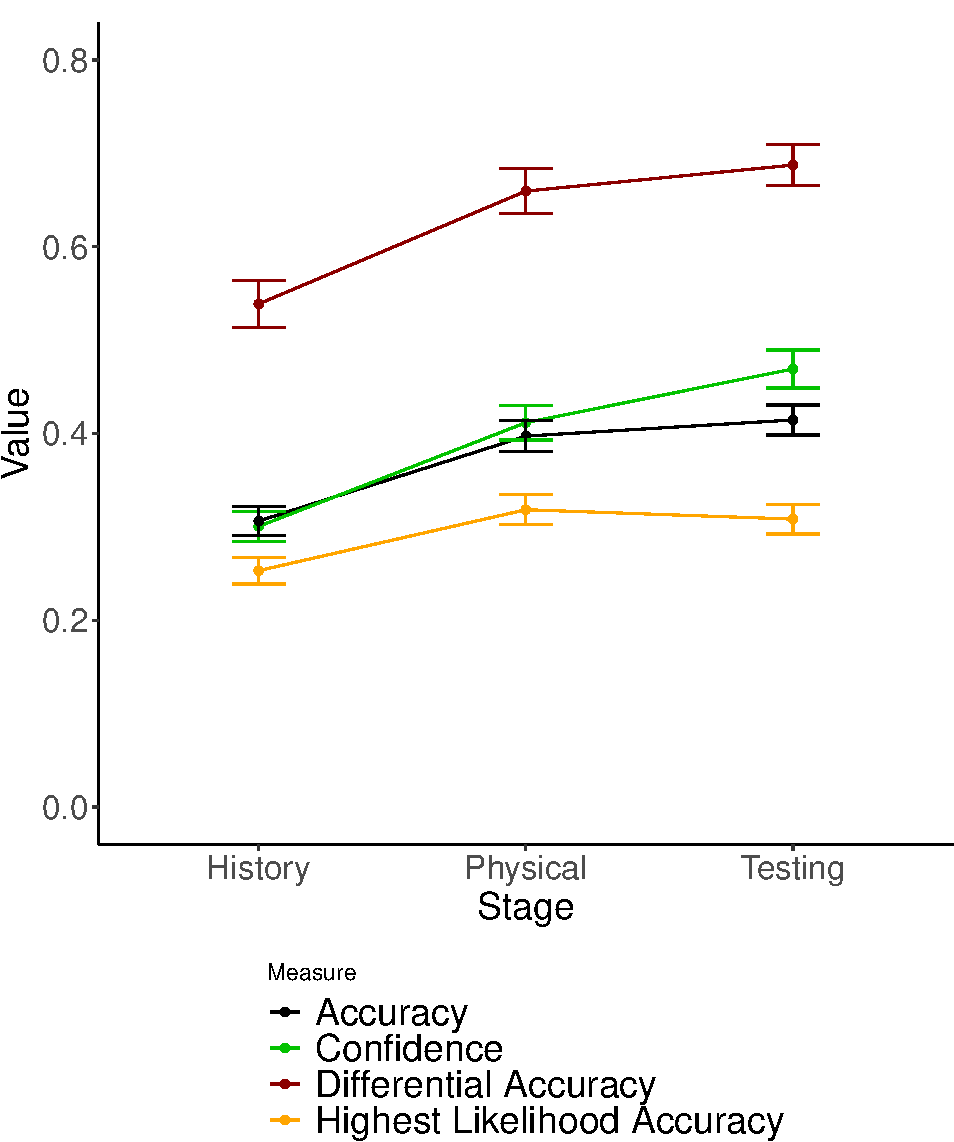
\includegraphics{_main_files/figure-latex/meyerGraph-1.pdf}

\emph{Figure 1: Graph showing Accuracy (black) and Confidence (green) at each of the three information stages.}

\hypertarget{differentials}{%
\subsection{Differentials}\label{differentials}}

We first look at the number of differentials that participants report at each stage. Participants overall increased the number of the differentials they reported as they received more information (F(1, 107) = 94.02, η\textsuperscript{2}G = .08, p \textless{} .001). Participants reported fewer differentials during the Patient History stage (M = 3.20, SD = 1.11) than during the Physical Examination (M = 3.88, SD = 1.33) and Testing stages (M = 4.12, SD = 1.43). The majority (74/85) did not decrease the number of differentials between Patient History and Testing on any case.

\begin{Shaded}
\begin{Highlighting}[]
\NormalTok{nPpts }\OtherTok{\textless{}{-}} \FunctionTok{nrow}\NormalTok{(studentAggData)}

\NormalTok{xb }\OtherTok{\textless{}{-}} \FunctionTok{c}\NormalTok{(}\FunctionTok{rep}\NormalTok{(}\StringTok{"Patient History"}\NormalTok{,nPpts),}\FunctionTok{rep}\NormalTok{(}\StringTok{"Physical Examination"}\NormalTok{,nPpts), }\FunctionTok{rep}\NormalTok{(}\StringTok{"Testing"}\NormalTok{,nPpts))}
\NormalTok{yb }\OtherTok{\textless{}{-}} \FunctionTok{c}\NormalTok{(studentAggData}\SpecialCharTok{$}\NormalTok{meanInitialDiffs, studentAggData}\SpecialCharTok{$}\NormalTok{meanMiddleDiffs, studentAggData}\SpecialCharTok{$}\NormalTok{meanFinalDiffs)}
\NormalTok{dataV }\OtherTok{\textless{}{-}} \FunctionTok{data.frame}\NormalTok{(}\StringTok{"Stage"} \OtherTok{=}\NormalTok{ xb, }\StringTok{"Mean"}\OtherTok{=}\NormalTok{ yb)}
\NormalTok{dataV}\SpecialCharTok{$}\NormalTok{Stage }\OtherTok{\textless{}{-}} \FunctionTok{as.factor}\NormalTok{(dataV}\SpecialCharTok{$}\NormalTok{Stage)}
\NormalTok{diffs }\OtherTok{\textless{}{-}} \FunctionTok{ggplot}\NormalTok{(dataV, }\FunctionTok{aes}\NormalTok{(}\AttributeTok{x=}\NormalTok{Stage, }\AttributeTok{y=}\NormalTok{Mean)) }\SpecialCharTok{+}
  \FunctionTok{geom\_violin}\NormalTok{(}\AttributeTok{colour=}\StringTok{"black"}\NormalTok{, }\AttributeTok{fill=}\NormalTok{differentialColour, }\AttributeTok{alpha=}\FloatTok{0.8}\NormalTok{, }\AttributeTok{trim=}\ConstantTok{FALSE}\NormalTok{) }\SpecialCharTok{+} 
  \CommentTok{\# geom\_dotplot(binaxis=\textquotesingle{}y\textquotesingle{}, stackdir=\textquotesingle{}center\textquotesingle{}, dotsize=0.5,colour="white") +}
  \FunctionTok{stat\_summary}\NormalTok{(}\AttributeTok{fun.data=}\NormalTok{data\_summary, }\AttributeTok{colour=}\StringTok{"red"}\NormalTok{)}

\FunctionTok{print}\NormalTok{(diffs }\SpecialCharTok{+}
        \FunctionTok{labs}\NormalTok{(}\AttributeTok{x =} \StringTok{"Stage"}\NormalTok{, }\AttributeTok{y =} \StringTok{"Average Differentials"}\NormalTok{) }\SpecialCharTok{+}
        \FunctionTok{theme\_classic}\NormalTok{() }\SpecialCharTok{+}
        \FunctionTok{theme}\NormalTok{(}\AttributeTok{axis.text=}\FunctionTok{element\_text}\NormalTok{(}\AttributeTok{size=}\DecValTok{16}\NormalTok{),}
               \AttributeTok{axis.title=}\FunctionTok{element\_text}\NormalTok{(}\AttributeTok{size=}\DecValTok{18}\NormalTok{),}
               \AttributeTok{plot.title=}\FunctionTok{element\_text}\NormalTok{(}\AttributeTok{size=}\DecValTok{18}\NormalTok{,}\AttributeTok{face=}\StringTok{"bold"}\NormalTok{),}
              \AttributeTok{line =} \FunctionTok{element\_blank}\NormalTok{()}
\NormalTok{        )}
\NormalTok{      ) }
\end{Highlighting}
\end{Shaded}

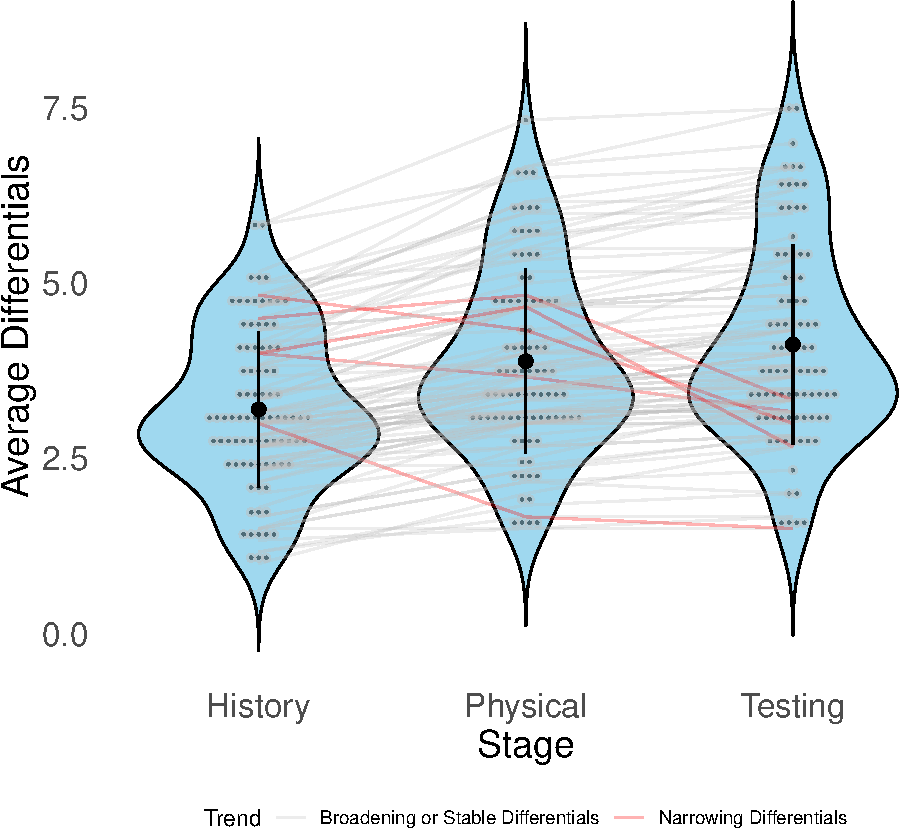
\includegraphics{_main_files/figure-latex/diffsOverStages-1.pdf}

\begin{Shaded}
\begin{Highlighting}[]
\DocumentationTok{\#\#\#dataV$Stage \textless{}{-} as.numeric(dataV$Stage)}
\DocumentationTok{\#\#\#model \textless{}{-} lm(Mean \textasciitilde{} Stage, data=dataV)}
\DocumentationTok{\#\#\#print(summary(model))}
\end{Highlighting}
\end{Shaded}

\emph{Figure 2: The average number of differentials after each stage of information seeking.}

To look at whether the number of initial differentials generated the amount of information sought, we conducted a Pearson's Correlation test on individual differences. We find an association (see Figure 3) between the average number of differentials generated from the Patient History and the average amount of information sought during cases (r(83) = 0.30, 95\% CI = {[}.10, .49{]}, p = .005). As previously discussed, participants rarely seem to remove differentials from consideration. Therefore, one can surmise here that higher information seeking is associated with the consideration of more diagnostic differentials.

\begin{Shaded}
\begin{Highlighting}[]
\DocumentationTok{\#\#\# Correlation between initial differentials and overall confidence change}

\NormalTok{cor }\OtherTok{\textless{}{-}} \FunctionTok{cor.test}\NormalTok{(studentAggData}\SpecialCharTok{$}\NormalTok{meanInitialDiffs,studentAggData}\SpecialCharTok{$}\NormalTok{proportionOfInfo,}\AttributeTok{method=}\StringTok{"pearson"}\NormalTok{)}

\NormalTok{diffCon }\OtherTok{\textless{}{-}} \FunctionTok{ggplot}\NormalTok{(}\AttributeTok{data =}\NormalTok{ studentAggData, }\FunctionTok{aes}\NormalTok{(}\AttributeTok{x=}\NormalTok{meanInitialDiffs, }\AttributeTok{y=}\NormalTok{proportionOfInfo)) }\SpecialCharTok{+}
  \FunctionTok{geom\_point}\NormalTok{() }\SpecialCharTok{+}
  \FunctionTok{geom\_smooth}\NormalTok{(}\AttributeTok{method=}\NormalTok{lm , }\AttributeTok{color=}\NormalTok{confidenceColour, }\AttributeTok{fill=}\StringTok{"\#69b3a2"}\NormalTok{, }\AttributeTok{se=}\ConstantTok{TRUE}\NormalTok{) }\SpecialCharTok{+}
  \FunctionTok{theme\_classic}\NormalTok{()}

\FunctionTok{print}\NormalTok{(diffCon }\SpecialCharTok{+} 
      \FunctionTok{labs}\NormalTok{(}\AttributeTok{y=}\StringTok{"Proportion of Possible Information Requested"}\NormalTok{, }\AttributeTok{x =} \StringTok{"Number of Initial Differentials"}\NormalTok{) }\SpecialCharTok{+}
      \FunctionTok{theme}\NormalTok{(}\AttributeTok{axis.text=}\FunctionTok{element\_text}\NormalTok{(}\AttributeTok{size=}\DecValTok{16}\NormalTok{),}
             \AttributeTok{axis.title=}\FunctionTok{element\_text}\NormalTok{(}\AttributeTok{size=}\DecValTok{16}\NormalTok{),}
             \AttributeTok{plot.title=}\FunctionTok{element\_text}\NormalTok{(}\AttributeTok{size=}\DecValTok{14}\NormalTok{,}\AttributeTok{face=}\StringTok{"bold"}\NormalTok{)}
\NormalTok{      ))}
\end{Highlighting}
\end{Shaded}

\begin{verbatim}
## `geom_smooth()` using formula = 'y ~ x'
\end{verbatim}

\includegraphics{_main_files/figure-latex/initialDiffsAgainstInfoSeeking-1.pdf}

\emph{Figure 3: Scatter plot showing the relationship between the number of initial differentials (x-axis) and the proportion of available information sought (y-axis). Each point represents a single student with both variables average across the six cases that each student performs. The x-axis refers to the average number of differentials that participants report in their list at the Patient History stage. The y-axis refers to the average proportion of available information sought, with each case containing 29 pieces of information across the Patient History, Physical Examination and Testing stages. The line of best fit is plotted using the geom\_smooth function in R with a linear model. The shaded region shows the 95\% confidence interval of the correlation.}

\hypertarget{information-seeking-1}{%
\subsection{Information Seeking}\label{information-seeking-1}}

The Proportion of Information Seeking decreased with each information stage (F(2, 151) = 122.0, η\textsuperscript{2}G = .30, p \textless{} .001). Participants sought more of the available information during the Patient History stage (M = 0.85, SD = 0.20) than during both during the Physical Examination (M = 0.59, SD = 0.24) and Testing stages (M = 0.50, SD = 0.22).

When conducting a Pearson's Product Correlation test, we do not find that participants who sought more information across cases were also more accurate in their diagnoses (r(83) = 0.17, 95\% CI = {[}-.04, .37{]}, p = .11). However, participants who sought more information did tend to increase their confidence more (r(83) = 0.24, 95\% CI = {[}.02, .43{]}, p = .03). This is distinct from their final confidence, for which we did not find evidence of an association with the amount of information sought (r(83) = 0.11, 95\% CI = {[}-.11, .31{]}, p = .33). While seeking more information may imbue students with a greater level of confidence, it does not necessarily translate into more accurate diagnoses. This links to the results presented in Figure 1, in which confidence and accuracy were related to one another but imperfectly (especially during the Testing stage).

\begin{Shaded}
\begin{Highlighting}[]
\DocumentationTok{\#\#\# Correlation between initial differentials and overall confidence change}

\NormalTok{cor }\OtherTok{\textless{}{-}} \FunctionTok{cor.test}\NormalTok{(studentAggData}\SpecialCharTok{$}\NormalTok{meanInitialDiffs,studentAggData}\SpecialCharTok{$}\NormalTok{meanConfidenceOverallChange,}\AttributeTok{method=}\StringTok{"pearson"}\NormalTok{)}

\NormalTok{diffCon }\OtherTok{\textless{}{-}} \FunctionTok{ggplot}\NormalTok{(}\AttributeTok{data =}\NormalTok{ studentAggData, }\FunctionTok{aes}\NormalTok{(}\AttributeTok{x=}\NormalTok{meanInitialDiffs, }\AttributeTok{y=}\NormalTok{meanConfidenceOverallChange)) }\SpecialCharTok{+}
  \FunctionTok{geom\_point}\NormalTok{() }\SpecialCharTok{+}
  \FunctionTok{geom\_smooth}\NormalTok{(}\AttributeTok{method=}\NormalTok{lm , }\AttributeTok{color=}\NormalTok{confidenceColour, }\AttributeTok{fill=}\StringTok{"\#69b3a2"}\NormalTok{, }\AttributeTok{se=}\ConstantTok{TRUE}\NormalTok{) }\SpecialCharTok{+}
  \FunctionTok{theme\_classic}\NormalTok{()}

\FunctionTok{print}\NormalTok{(diffCon }\SpecialCharTok{+} 
      \FunctionTok{labs}\NormalTok{(}\AttributeTok{y=}\StringTok{"Final Confidence {-} Initial Confidence"}\NormalTok{, }\AttributeTok{x =} \StringTok{"Number of Initial Differentials"}\NormalTok{) }\SpecialCharTok{+}
      \FunctionTok{theme}\NormalTok{(}\AttributeTok{axis.text=}\FunctionTok{element\_text}\NormalTok{(}\AttributeTok{size=}\DecValTok{16}\NormalTok{),}
             \AttributeTok{axis.title=}\FunctionTok{element\_text}\NormalTok{(}\AttributeTok{size=}\DecValTok{16}\NormalTok{),}
             \AttributeTok{plot.title=}\FunctionTok{element\_text}\NormalTok{(}\AttributeTok{size=}\DecValTok{14}\NormalTok{,}\AttributeTok{face=}\StringTok{"bold"}\NormalTok{)}
\NormalTok{      ))}
\end{Highlighting}
\end{Shaded}

\begin{verbatim}
## `geom_smooth()` using formula = 'y ~ x'
\end{verbatim}

\includegraphics{_main_files/figure-latex/initialDiffsAgainstConfidence-1.pdf}

\emph{Figure 4: Scatter plot showing the relationship between the number of initial differentials (x-axis) and the proportion of available information sought (y-axis). Each point represents a single student with both variables average across the six cases that each student performs. The x-axis refers to the average number of differentials that participants report in their list at the Patient History stage. The y-axis refers to the difference in confidence between the final stage (Testing) and the first stage (Patient History). The line of best fit is plotted using the geom\_smooth function in R with a linear model. The shaded region shows the 95\% confidence interval of the correlation.}

The amount of information sought does not seem to be predictive of accuracy. However, it may be the case that patterns of information sought are instead predictive of differences in accuracy on this task. In order to test this, we investigate whether information seeking is predictive of participants who are higher or lower in their diagnostic accuracy using binary classification and receiver operating characteristic (ROC) analysis. We trained a binary classification algorithm using a generalised logistic regression model to identify if participants of high or low accuracy based on the information they sought. We split all cases by whether they performed by a high and low Accuracy participant using a median split of participants by their average Accuracy across the six cases. We train the classifier using a Generalised Linear Model (GLM) by treating the 29 binary variables for each information as predictors (with a 1 signifying that the information was sought for that case and 0 when the information was not sought) to predict the binary outcome of whether the participant is a low or high accuracy participant. We used Leave One Out Cross Validation, such that each case is predicted by training the algorithm on all other cases. By plotting an ROC curve of our classifier, we find an area under the curve (AUC) value of 0.72 (plotted in Figure 5). When conducting a DeLong test, to test the null hypothesis that the AUC is equal is 0.5 (i.e.~that the classifier is completely unable to predict high and low accuracy participants), we find p \textless{} .001, indicating that the AUC differs significantly from 0.5 and that the classifier is able to reliably predict high and low accuracy participants.

This indicates overall that differences in information seeking are indeed predictive of a difference in participant ability at above chance at a broad level. Essentially, information seeking patterns separate high and low accuracy participants, but this analysis does not tell us what aspects of information seeking in particular are predictive of accuracy. We next seek to identify and better characterise these specific differences in information seeking that contribute to this relationship with diagnostic ability by correlating behavioural information seeking variables with accuracy.

\begin{Shaded}
\begin{Highlighting}[]
\FunctionTok{set.seed}\NormalTok{(}\DecValTok{1000}\NormalTok{)}

\NormalTok{classifierData }\OtherTok{\textless{}{-}}\NormalTok{ infoSeekingFullMatrix[,}\FunctionTok{c}\NormalTok{(}\DecValTok{2}\SpecialCharTok{:}\DecValTok{29}\NormalTok{,}\DecValTok{38}\NormalTok{)]}
\NormalTok{classifierData}\SpecialCharTok{$}\NormalTok{AccuracyGroup }\OtherTok{\textless{}{-}} \FunctionTok{as.integer}\NormalTok{(}\FunctionTok{as.logical}\NormalTok{(classifierData}\SpecialCharTok{$}\NormalTok{AccuracyGroup}\SpecialCharTok{\textgreater{}}\DecValTok{2}\NormalTok{))}
\NormalTok{classifierData}\SpecialCharTok{$}\NormalTok{AccuracyGroup }\OtherTok{\textless{}{-}} \FunctionTok{as.factor}\NormalTok{(classifierData}\SpecialCharTok{$}\NormalTok{AccuracyGroup)}
\FunctionTok{colnames}\NormalTok{(classifierData)[}\DecValTok{1}\SpecialCharTok{:}\DecValTok{29}\NormalTok{] }\OtherTok{\textless{}{-}} \FunctionTok{c}\NormalTok{(}\StringTok{"T2"}\NormalTok{,  }\StringTok{"T3"}\NormalTok{,  }\StringTok{"T4"}\NormalTok{,  }\StringTok{"T5"}\NormalTok{,  }\StringTok{"T6"}\NormalTok{,  }\StringTok{"T7"}\NormalTok{,  }
                                      \StringTok{"T8"}\NormalTok{,  }\StringTok{"T9"}\NormalTok{, }\StringTok{"T10"}\NormalTok{, }\StringTok{"T11"}\NormalTok{, }\StringTok{"T12"}\NormalTok{, }\StringTok{"T13"}\NormalTok{, }\StringTok{"T14"}\NormalTok{, }
                                      \StringTok{"T15"}\NormalTok{, }\StringTok{"T16"}\NormalTok{, }\StringTok{"T17"}\NormalTok{, }\StringTok{"T18"}\NormalTok{, }\StringTok{"T19"}\NormalTok{, }\StringTok{"T20"}\NormalTok{, }\StringTok{"T21"}\NormalTok{, }\StringTok{"T22"}\NormalTok{, }
                                      \StringTok{"T23"}\NormalTok{, }\StringTok{"T24"}\NormalTok{, }\StringTok{"T25"}\NormalTok{, }\StringTok{"T26"}\NormalTok{, }\StringTok{"T27"}\NormalTok{, }\StringTok{"T28"}\NormalTok{, }\StringTok{"T29"}\NormalTok{,}\StringTok{"Group"}\NormalTok{)}


\NormalTok{thresh}\OtherTok{\textless{}{-}}\FunctionTok{seq}\NormalTok{(}\DecValTok{0}\NormalTok{,}\DecValTok{1}\NormalTok{,}\FloatTok{0.001}\NormalTok{)}
\CommentTok{\#specify the cross{-}validation method}
\NormalTok{ctrl }\OtherTok{\textless{}{-}} \FunctionTok{trainControl}\NormalTok{(}\AttributeTok{method =} \StringTok{"LOOCV"}\NormalTok{, }\AttributeTok{savePredictions =} \ConstantTok{TRUE}\NormalTok{)}

\CommentTok{\# Shuffle rows in case there are order biases}
\NormalTok{classifierData }\OtherTok{\textless{}{-}}\NormalTok{ classifierData[}\FunctionTok{sample}\NormalTok{(}\DecValTok{1}\SpecialCharTok{:}\FunctionTok{nrow}\NormalTok{(classifierData)),]}
\NormalTok{modelglm}\OtherTok{\textless{}{-}}\FunctionTok{train}\NormalTok{(Group }\SpecialCharTok{\textasciitilde{}}\NormalTok{ T2 }\SpecialCharTok{+}\NormalTok{ T3 }\SpecialCharTok{+}\NormalTok{ T4 }\SpecialCharTok{+}\NormalTok{ T5 }\SpecialCharTok{+}\NormalTok{ T6 }\SpecialCharTok{+}\NormalTok{ T7 }\SpecialCharTok{+}\NormalTok{ T8 }\SpecialCharTok{+}\NormalTok{ T9 }\SpecialCharTok{+}\NormalTok{ T10 }\SpecialCharTok{+}
\NormalTok{                T11 }\SpecialCharTok{+}\NormalTok{ T12 }\SpecialCharTok{+}\NormalTok{ T13 }\SpecialCharTok{+}\NormalTok{ T14 }\SpecialCharTok{+}\NormalTok{ T15 }\SpecialCharTok{+}\NormalTok{ T16 }\SpecialCharTok{+}\NormalTok{ T17 }\SpecialCharTok{+}\NormalTok{  T18 }\SpecialCharTok{+}\NormalTok{ T19 }\SpecialCharTok{+}\NormalTok{ T20 }\SpecialCharTok{+}
\NormalTok{                T21 }\SpecialCharTok{+}\NormalTok{ T22 }\SpecialCharTok{+}\NormalTok{ T23 }\SpecialCharTok{+}\NormalTok{ T24 }\SpecialCharTok{+}\NormalTok{ T25 }\SpecialCharTok{+}\NormalTok{ T26 }\SpecialCharTok{+}\NormalTok{ T27 }\SpecialCharTok{+}\NormalTok{ T28 }\SpecialCharTok{+}\NormalTok{ T29, }\AttributeTok{method =} \StringTok{"glm"}\NormalTok{, }\AttributeTok{family =} \FunctionTok{binomial}\NormalTok{(}\AttributeTok{link=}\NormalTok{probit), }\AttributeTok{data =}\NormalTok{ classifierData, }\AttributeTok{trControl =}\NormalTok{ ctrl)}
\NormalTok{prediglm}\OtherTok{\textless{}{-}}\FunctionTok{predict}\NormalTok{(modelglm,}\AttributeTok{type =} \StringTok{"prob"}\NormalTok{)[}\DecValTok{2}\NormalTok{]}

\CommentTok{\# Plot all test results on one ROC curve}
\NormalTok{rocPlot }\OtherTok{\textless{}{-}} \FunctionTok{roc.plot}\NormalTok{(}\AttributeTok{x=}\NormalTok{classifierData}\SpecialCharTok{$}\NormalTok{Group}\SpecialCharTok{==}\StringTok{"1"}\NormalTok{,}\AttributeTok{pred=}\FunctionTok{cbind}\NormalTok{(prediglm),}\AttributeTok{legend =}\NormalTok{ T,}
                    \AttributeTok{leg.text =} \FunctionTok{c}\NormalTok{(}\StringTok{"GLM"}\NormalTok{),}\AttributeTok{thresholds =}\NormalTok{ thresh)}\SpecialCharTok{$}\NormalTok{roc.vol}
\end{Highlighting}
\end{Shaded}

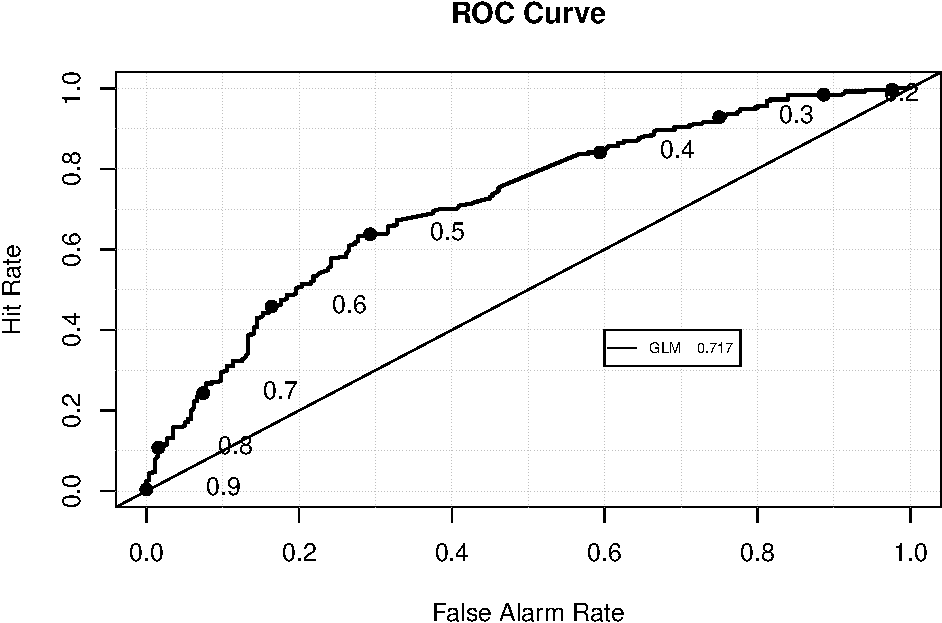
\includegraphics{_main_files/figure-latex/accuracyClassifier-1.pdf}

\emph{Figure 5: Receiver-Operator Characteristic (ROC) curve using a Generalised Linear Model to classify individual cases as being performed by either high or low accuracy participants. The models are trained on the raw binary predictor variables for each of the 29 available pieces of information, with 0 indicating that the information was not sought for the case and 1 indicating that the information was sought. Participants were sorted as high and low accuracy based on a median split on their average Accuracy value across the six cases.}

In order to examine more specifically what differences in information seeking are driving differences in both accuracy and confidence, we look at the relationship between accuracy and informational value. We assess the degree to which each participant's accuracy is predicted by the quality of the information they sought and find evidence for a positive relationship between accuracy and information value (r(83) = 0.25, 95\% CI = {[}.04, .44{]}, p = .02), as well as between confidence and information value (r(83) = 0.28, 95\% CI = {[}.07, .47{]}, p = .01).

\hypertarget{discussion}{%
\section*{Discussion}\label{discussion}}
\addcontentsline{toc}{section}{Discussion}

This study of 85 medical students found that accuracy and confidence are well calibrated. Previous work (e.g.~Meyer et al., 2011) have noted a gap between subjective confidence and objective accuracy. In particular, there has been demonstrated to be a general tendency for less experienced medical trainees to be underconfident and for more experienced medical professionals to be overconfident (Yang and Thompson, 2010). Part of this discrepancy between our findings and past findings could stem from the diagnostic uncertainty expressed by students in this study, which they do in two ways. Firstly, students broaden, rather than narrow, their considered diagnostic differentials with more information and still report a broad range of differentials after receiving all available information for a given case. There is a general adage in healthcare that medical students come across which says that ``history is 80\% of the diagnosis''. It is therefore worth considering whether there is a specific facet of diagnostic decisions whereby students are taught not to disregard diagnostic possibilities easily. Secondly, students reported fairly low confidence overall to treat patients, with an average confidence of below 50\% even after receiving all available information. This may indicate that part of ensuring appropriate confidence, or expressions of uncertainty could be related to properly evaluating all possible diagnostic differentials rather than forcing decisions to focus on a single diagnosis, which has been cited previously as a problematic tendency (Redelmeier \& Shafir, 2023).

We find the amount of information sought informed confidence, whilst accuracy was associated with seeking more useful information on each case. This hints at the richness of this dataset in picking on information seeking and differential generation behaviour. We note however that whilst predictors of diagnostic by information seeking behaviour were found, they do not tell us how overarching differences in such behaviour arise. One possibility is that these differences stem from reasoning strategies that we cannot infer from this current dataset. In order to ascertain these strategies, we conduct a follow-up study using a similar diagnostic paradigm conducted in-person where students think out loud as they make diagnoses. We use criteria taken from Coderre et al.~(2003) to code case by the reasoning strategy employed. We hypothesise that different reasoning strategies for generating differentials are useful for some cases more than others and that information seeking varies as a function of strategy. This coding of reasoning strategies is then subsequently used to classify the same reasoning strategies in the online dataset from study 1 (where we do not have access to the participants' thought process) by using the information they sought.

\hypertarget{study-3---diagnostic-reasoning-strategies-via-a-think-aloud-paradigm}{%
\chapter*{Study 3 - Diagnostic Reasoning Strategies via a Think-Aloud Paradigm}\label{study-3---diagnostic-reasoning-strategies-via-a-think-aloud-paradigm}}
\addcontentsline{toc}{chapter}{Study 3 - Diagnostic Reasoning Strategies via a Think-Aloud Paradigm}

\adjustmtc
\markboth{Think Aloud}{}

We aimed to replicate the finding of considered differentials increasing with more information when the method by which these differentials were reported. Are students seeking information to confirm their existing set of differentials, to rule out differentials or to expand their set of considered possibilities? And are these different approaches interleaving or are they more dependent on individual diagnostic decision making styles? In order to provide more context to the results from study 1, we conducted a follow-up study that utilised a very similar experimental procedure, but instead prompted students to think out loud as they were performing the task. and the transcripts were coded to conduct both quantitative and qualitative analysis.

Think-aloud methodologies are useful for directly accessing ongoing thought processes during decisions (van Someren, Barnard \& Sandberg, 1994). The use of thinking aloud (or verbal protocols) in research is useful for being able to access the information attended to participants in short term memory (Payne, 1994) and can be treated as the ongoing behavioural state of a participant's knowledge (Newell \& Simon, 1972). Think-aloud protocols have historically been used to study problem solving, particularly for comparing how novices and experts solve problems such as finding the best move in chess (de Groot, 1946, Bilalić, McLeod \& Gobet, 2008). Diagnosis is a decisional process that develops over time and allowing participants to think aloud reflects this by providing a time-ordered sequence of how thought processes develop (Payne, 1994). This is especially well-suited to our task where the information available to participants is controlled with time, allowing us to investigate how diagnostic thinking develops with more information. A think-aloud methodology has previously been used to study the differences between novice and expert clinicians during diagnostic reasoning (Coderre et al., 2003). This study found a general trend that experts tend to use a `pattern recognition' approach to diagnosis more than novices, who tended to use a `hypothetico-deductive' process (which is aforementioned to be the `textbook' description of the diagnostic process), but this was highly dependent on the case presented. We build on the work of Coderre et al.~(2003) here to further investigate how reasoning strategies contribute to accuracy and why certain cases result in differing strategies.

\hypertarget{methods-1}{%
\section*{Methods}\label{methods-1}}
\addcontentsline{toc}{section}{Methods}

\hypertarget{participants-1}{%
\subsection*{Participants}\label{participants-1}}
\addcontentsline{toc}{subsection}{Participants}

16 participants were recruited for this study. Participants were 5th or 6th year medical students at Oxford University (including 2nd year Oxford University Graduate Entry Medical students) recruited via posters in the John Radcliffe Hospital in Oxford and via a mailing list for students managed by the Medical Sciences Division at the University of Oxford. The study was conducted onsite at John Radcliffe hospital. Participants were recruited between July 5th 2023 and December 1st 2023. Data was reviewed on an ongoing basis to cease recruitment when emerging themes were exhausted. This study was reviewed and granted ethical approval as an amendment to our existing protocol to allow for audio recordings by the Oxford Medical Sciences Interdivisional Research Ethics Committee under reference R81158/RE004.

\hypertarget{materials-1}{%
\subsection*{Materials}\label{materials-1}}
\addcontentsline{toc}{subsection}{Materials}

The same set of cases and a similar computer interface from Study 1 were used for this study, with the exception that participants no longer recorded their differentials in a specific screen at the end of each information gathering stage. Instead, participants' differentials were recorded as a more naturalistic part of their diagnostic process as they reported aloud their thoughts as they worked through each diagnostic case. The study was conducted onsite using a laptop, with actions on screen recorded on video and the audio of participants' thinking aloud recorded via a microphone. Informed consent was obtained anonymously using an online electronic information sheet and consent form. Information, including experimental data and audio recordings, collected during the study were stored under anonymised IDs with no linkages to participants. Data was kept on a password-protected computer and hard drive.

\hypertarget{procedure-1}{%
\subsection*{Procedure}\label{procedure-1}}
\addcontentsline{toc}{subsection}{Procedure}

The general procedure was very similar to that of Study 1, except that participants were given the following instructions at the start of the study:

\emph{``Whilst you are doing the task, you will be asked to think aloud. This means that you verbalise what you are thinking about, especially how you interpret the information you receive and what conditions or diagnoses you are considering or are concerned about for each patient case. If you have nothing to say or nothing on your mind, there's no need to say anything but do say whatever is on your mind once it pops up. If you are unsure about anything you see or do not know about what something means, you will not receive any help but verbalise when you are unsure about anything during the task. Please make sure that you speak clearly `to the room'.''}

The experimenter occasionally prompted participants with content-neutral probes: \emph{``can you tell me what you are thinking?''} in cases of periods of long silence, and \emph{``can you tell me more?''} when the participant said something vague that may warrant further detail. We emphasise that these are non-leading questions. The audio of the participants' verbalisations was recorded and then transcribed. An initial transcript was generated using Microsoft Office's transcription feature, but the transcript was checked and modified for accuracy by listening through the audio recordings again. The screen of the experimental interface was also recorded, such that the audio could be linked to specific actions within the task. The focus of this study is on verbal utterances rather than any non-verbal or inferential aspects of the participants' qualitative data. At the end of the experiment, the researcher administered a semi-structured interview to better understand what the participants feel their diagnostic reasoning approach tends to be. These questions are provided in the Appendices.

\hypertarget{data-analysis-1}{%
\subsection*{Data Analysis}\label{data-analysis-1}}
\addcontentsline{toc}{subsection}{Data Analysis}

We conducted a theory-driven semantic thematic analysis (as per definitions detailed by Braun and Clarke, 2006) to code utterances under specific categories. This kind of thematic analysis is suitable given that our qualitative data is from a structured experiment, rather than a dataset with a looser structure (e.g.~interview recordings). As a result, we apply deductive analysis using predetermined codes for think-aloud utterances and for a debrief interview where we administer a semi-structured interview with specific questions of interest.

Firstly, we code all utterances related to the main research areas of interest in this project, namely information seeking, confidence and differential/hypothesis generation. Respectively, we define the following codes:

\begin{itemize}
\item
  \textbf{Differential Evaluation}: any time that the participant (each of the following is considered a separate subcode):
\item
  \begin{itemize}
  \tightlist
  \item
    \emph{Differential Added:} - Mentions a new condition that they are considering
  \end{itemize}
\item
  \begin{itemize}
  \tightlist
  \item
    \emph{Differential Removed:} - Rules out or eliminates a condition from consideration
  \end{itemize}
\item
  \begin{itemize}
  \tightlist
  \item
    \emph{Likelihood Increased:} - Mention of increased likelihood of a previously mentioned condition, or that information seems to correspond with a condition
  \end{itemize}
\item
  \begin{itemize}
  \tightlist
  \item
    \emph{Likelihood Decreased:} - Mention of decreased likelihood of a previously mentioned condition, or that information seems to contradict with a condition
  \end{itemize}
\item
  \textbf{Information Seeking Strategies}: any time the participant expresses why they may or may not request a particular piece of information in relation to ruling out or confirming a condition.
\end{itemize}

We also define a group of codes that indicate three different diagnostic reasoning strategies: hypothetico-deductive reasoning, scheme-inductive reasoning and pattern recognition (Coderre et al.., 2003). These were defined as follows:

\begin{itemize}
\tightlist
\item
  \textbf{Hypothetico-Deductive Reasoning} - prior to selecting the most likely diagnosis, the participant analysed any alternative differentials one by one through something akin to a process of elimination.
\item
  \textbf{Scheme Inductive Reasoning} - participant structures their diagnosis by pathophysiological systems or categories of conditions (e.g., infective vs cardiovascular causes) to determine root causes of patient symptoms rather than focusing on specific conditions.
\item
  \textbf{Pattern Recognition} - participant considers only a single diagnosis with only perfunctory attention to the alternatives, or makes reference to pattern matching when using a prototypical condition to match its symptoms against the current observed symptoms for the patient (e.g., ``these symptoms sound like X'' or ``this fits with a picture of Y'').
\end{itemize}

We first code specific statements within each case that suggested one of these strategies, and then determined which strategy was most prevalent or influential for cases as a whole such that each case was categorised under one of these strategies. In addition to coding each case under one of these strategies, we also code participants on an overall level based on their subjective perception of how they make diagnostic decisions. This is based on responses provided during the debrief interview (as described in the Procedure section). Hence, reasoning strategy codes are at the case level and also at the participant level.

Coding of utterances and case-wise reasoning strategies were conducted with a second independent coder. For reasoning strategies, initial interrater reliability was low, with both coders agreeing on 58.3\% of cases. Conflict resolution led to changes made to the coding criteria by prioritising strategies used early in a case, as some participants were noted to utilise multiple strategies within a single case, as well as allowing some cases to be coded as not having a clear strategy due to a lack of utterances. Conflicts were then resolved with these updated criteria. Both coders agreed on 78\% of cases when coding for correctness, with conflicts resolved in consultation with a member of expert panel used to develop the vignettes (as mentioned in Study 1).

Although we do not record differentials in the same way as in Study 1 (in a list with corresponding likelihood and severity ratings), we do obtain the other variables. Namely, we record confidence at each stage of information seeking and data around the information sought by participants. As we do not explicitly record differentials in the same manner as in Study 1, accuracy is operationalised differently. We code each case as `correct' if a correct differential is mentioned at some point by the participant (using the same marking scheme, found in the Appendices).

\hypertarget{results-1}{%
\section*{Results}\label{results-1}}
\addcontentsline{toc}{section}{Results}

First, we look at overall quantitative characteristics of the think aloud statements. When looking at accuracy (the proportion of cases where a correct differential was mentioned by the participant), accuracy was 0.57 across all cases. This varied considerably by condition however, with accuracy across participants for each condition being as follows: AD = 0.63, GBS = 0.88, MTB = 0.19, TA = 0.44, TTP = 0.69, UC = 0.63. For utterances coded as Differential Evaluations, participants on average made 5.21 such utterances per case (SD = 2.80). The mean number of Differential Evaluations was relatively constant by condition except for the AD case: AD = 8.18, GBS = 4.63, MTB = 4.81, TA = 4.75, TTP = 4.25, UC = 4.63. Participants varied in how much they spoke during the study, uttering 1038-7730 words (M = 4194) across the scenarios. Part of this range is driven by participants repeating information they see during the task, but participants also varied in terms of how much they externalised their thought process.

As previously mentioned, Differential Evaluations can be further categorised into one of four subcodes: Differential Added, Differential Removed, Likelihood Increased and Likelihood Decreased. As found in the previous study, there is a general reticence to disregard differentials completely. Participants expressed significantly more statements adding differentials (M = 3.14, SD = 0.89) than removing differentials (M = 0.27, SD = 0.28) (t(15) = 14.14, MDiff = 2.86, p \textless{} .001). Participants expressed more statements of decreasing likelihoods (M = 0.99, SD = 0.62) rather than increasing likelihoods (M = 0.93, SD = 0.46) but we did not find evidence of a significant difference (t(15) = 0.34, MDiff = 0.06, p = .73).

\hypertarget{reasoning-strategies}{%
\subsection*{Reasoning Strategies}\label{reasoning-strategies}}
\addcontentsline{toc}{subsection}{Reasoning Strategies}

Next we look at our coding of reasoning strategies at a case level. As mentioned, our criteria for each code was applied to each individual case based on the transcribed utterances. When looking at reasoning strategies by case, 43 cases were coded as Hypothetico-Deductive, 29 were coded as Pattern Recognition and 18 were coded as Scheme Inductive (the remainder of cases did not contain enough clear utterances to classify under one of these strategies). Accuracy was higher for cases coded as Hypothetico-Deductive (71\%) compared to both Pattern Recognition cases (64\%) and Scheme Inductive (39\%). It is worth noting here that accuracy was solely based on participants mentioning differentials during their thinking aloud, which is naturally not facilitated by Scheme Inductive reasoning due to its focus on identifying pathophysiological systems acting as sources of patient symptoms rather than specific conditions. This can hence explain the lower `accuracy' for Scheme Inductive cases. We also note that the types of reasoning strategy used varies by condition (see Figure 13 below), with the MTB and TTP cases in particular exhibiting higher usage of Pattern Recognition than others. This could be because this case was considered harder than others and hence participants could not generate a larger set of candidate differentials due to its difficulty.

We note, rather unsurprisingly, that we observe a higher number of average Differential Evaluations when cases are correct (M = 5.85, SD = 0.38) compared to when they are incorrect (M = 4.34, SD = 0.39). Given our methodology for defining accuracy, participants are more likely to mention a correct differential if they mention more differentials. The procedure used in the previous study for collecting data on which differentials participants were considering at each information stage was not present here and hence we are not able to operationalise accuracy in the same manner as before. While we look at which differentials are mentioned, we cannot observe how participants weigh up differentials against each other in the same way as in the first study.

To connect the results of this study to those of Study 1, we break down the same dependent variables (as operationalised in that study) by reasoning strategy. We do not apply statistics to this study due to the lower sample size. We first categorise each of the 6 cases as having a `dominant' reasoning strategy based on which was utilised the most across participants. Through this process, we categorise three conditions as HD (AD, UC, GBS), three conditions as PR (MTB, TTP, TA). The proportions of participants who use each reasoning strategy for each condition can be viewed in Figure 10. We then compare the individual case classifications of strategy to this reasoning strategy that is most commonly used for that medical condition. Table 2 shows how dependent variables are affected by reasoning strategy. We find that the amount of information seeking was fairly consistent across reasoning strategy, but that PR cases were associated with higher value in information seeking. In order to derive informational value, we used the same values of each piece of information for each case that were derived in Study 1. This higher informational value does not translate into higher accuracy for PR cases, though we should note that the manner in which accuracy was defined for this study limits the analysis only to statements made out loud of specific conditions rather than formally recorded differentials as we did in Study 1. In order to formally replicate this finding with the larger dataset, we use the cases from this study and the coding of strategies to apply the same coding to our online dataset from Study 1.

\hypertarget{reasoning-strategies-in-study-1-dataset}{%
\subsection*{Reasoning Strategies in Study 1 Dataset}\label{reasoning-strategies-in-study-1-dataset}}
\addcontentsline{toc}{subsection}{Reasoning Strategies in Study 1 Dataset}

In order to apply reasoning strategies to the data from Study 1, we train a classifier using penalised multinomial regression to classify cases as HD, PR or SI using the cases from the think aloud study (with Leave One Out Cross Validation). The input parameters for the classifier are the 29 pieces of information as binary predictors (similar to the approach depicted in Figure 7) and the cases' condition. In other words, the cases from the think-aloud study make up the training data for the classifier whilst the cases from the larger online study is the test dataset. The classifier was implemented using R's nnet package (version 7.3-19). The testing data is then labelled with predicted testing strategies using R's predict function. We note that the training data was initially labelled with reasoning strategies using the think-aloud utterances and thus is separated from the information sought during the case.

We show a breakdown of cases by their coded reasoning strategy in Table 4. We now look to compare our key dependent variables by strategy, in particular comparing PR and HD cases. In line with our expectations based on the definitions of HD and PR reasoning approaches, we find that HD cases are associated with more differentials being considered (M = 3.37, SD = 1.64) average when compared to PR cases (M = 2.84, SD = 1.58) and find evidence of a difference between the two via a Welch Two Sample t-test (t = 2.89, MDiff = 0.53, p = .004). We find that PR cases are associated with higher informational value (M = 2.35, SD = 1.07) when compared to HD cases (M = 2.15, SD = 1.32) (t = 1.48, MDiff = 0.20, p = .14). However we do find evidence of higher amounts of information seeking for HD cases (M = 0.63, SD = 0.21) when compared to PR cases (M = 0.50, SD = 0.21), (t = 5.28, MDiff = 0.13, p \textless{} .001). Overall, this indicates that PR reasoning were associated with lower but more selective information seeking when compared to HD reasoning.

We hypothesised that an interaction with reasoning strategy is associated with accuracy on the task. This is because a single reasoning strategy is considered unlikely to be more accurate for all cases. As indicated by Figure 10, different patient conditions seem to result in varying reasoning strategies being utilised, which begs the question of what properties of a condition contribute to changes in strategy and in accuracy. One possibility is that reasoning strategy interacts with the diagnostic uncertainty of a case (i.e.~the breadth of conditions that a patient could have given their current symptoms and history, with some conditions presenting in a more apparent way than others), as captured by the number of initial differentials reported by participants. To test this hypothesis, we fit a linear model to predict accuracy with an interaction between the number of initial diagnoses and reasoning strategy.

\hypertarget{study-4---diagnostic-uncertainty-and-information-seeking-in-virtual-reality-paediatric-scenarios}{%
\chapter*{Study 4 - Diagnostic Uncertainty and Information Seeking in Virtual Reality Paediatric Scenarios}\label{study-4---diagnostic-uncertainty-and-information-seeking-in-virtual-reality-paediatric-scenarios}}
\addcontentsline{toc}{chapter}{Study 4 - Diagnostic Uncertainty and Information Seeking in Virtual Reality Paediatric Scenarios}

\adjustmtc
\markboth{VR Study}{}

A critique with the vignette task used in the previous studies is its lack of naturalism. For a start, participants are unable to see the patient, which is important given that the visual state (or distress) of a patient can be informative for a doctor in diagnosing the patient. In addition, the task is static in time, in that the patient does not change over the course of a case (i.e.~improving or deteriorating over time). The case also does not include any aspect of treatment of patients, where doctors can start managing the patient's symptoms and even using reactions to their treatment plan in order to change their understanding of the patient. In order to address these shortcomings in realism of our task, we used a virtual reality (VR) paradigm in order to investigate questions of differential evaluation, confidence and information seeking in a more naturalistic manner.

\hypertarget{methods-2}{%
\section*{Methods}\label{methods-2}}
\addcontentsline{toc}{section}{Methods}

\hypertarget{participants-2}{%
\subsection*{Participants}\label{participants-2}}
\addcontentsline{toc}{subsection}{Participants}

\hypertarget{materials-2}{%
\subsection*{Materials}\label{materials-2}}
\addcontentsline{toc}{subsection}{Materials}

We used VR scenarios implemented by Oxford Medical Simulation (OMS), a company that uses VR for medical education and simulation, in their bespoke software. Participants in this study were medical students based in Oxford who were at the time taking part in VR-based teaching sessions as part of their medical degrees. Students performed the scenarios using Oculus Quest 2 VR headsets. Scenarios were based in paediatrics, meaning that the patients in the scenario were children who were attending the hospital with their legal guardian. Each scenario features a visual 3D implementation of a basic ward room in a hospital. Participants are shown a (child) patient, their guardian and a nurse who can help with certain treatment and testing. All of the `avatars' in the scenario can be questioned by the participant using a predefined set of requests/actions (e.g.~asking the nurse to check blood pressure, asking the patient/child about if they are in pain). The scenarios have full sound (e.g.~being able to hear the patient's lung auscultation) and the avatars are voiced.

Each participant completed two scenarios over two separate VR sessions. The sessions were held around one month apart. During each session, the participants each performed one scenario in VR and observed their partner during their scenario. Participants also engaged in peer-to-peer feedback discussions as part of their education. The scenarios presented in each sessions are described below (students are split into two groups, shown below as groups A and B, each performing a different pair of scenarios in a fixed order):

Session One:
* Group A: patient/child is a 6-year-old-girl presenting with a 1 day history of central abdominal pain and thirst. She was generally unwell for 2 days prior, with reduced appetite and a sore throat. Collateral history reveals Type 1 Diabetes and erratic blood sugars. (True Condition: Diabetic Ketoacidosis)
* Group B: patient/child is a 5-year-old boy presenting with worsening shortness of breath, wheeze, and signs of respiratory distress, on the background of 2 days of likely viral illness. He has a medical history of asthma and has had similar exacerbations in the past. (True Condition: Acute Severe Exacerbation of Asthma)

Session Two:
* Group A: patient/child is a 5-year-old boy presenting with shortness of breath and drowsiness (True Condition: Chest Sepsis/Pneumonia)
* Group B: patient/child is a 5-year-old girl with a 1 day history of sore throat and fever. She starts having a generalised tonic clonic seizure during the scenario. (True Condition: Febrile seizure on background of tonsillitis)

\hypertarget{procedure-2}{%
\subsection*{Procedure}\label{procedure-2}}
\addcontentsline{toc}{subsection}{Procedure}

The aim for students in the scenarios was to diagnose the patient, begin treatment and hand over the case to a senior with appropriate understanding of the patient (handovers were conducted using a standardised framework known as SBAR, meaning that clinicians have to brief the senior on the Situation, Background, Assessment and Recommendation for the patient). Whilst in the scenario, participants can learn about the patient's medical history, check key parameters (such as temperature, pulse, blood pressure, respiratory rate etc), perform physical exams/tests and begin certain treatment actions (such as administering oxygen or prescribing medication). Compared to the previous studies, participants have a much wider array in terms of the information and tests they can request, as well as being able to begin a treatment plan.

After 5 minutes in the scenario (by which point it is expected that participants would have a history of the patient and have started some early assessment of the patient), participants are asked to pause the scenario (taking off their VR headset) and fill in a brief questionnaire on paper. Multiple VR participants were performing the scenario simultaneously and were paired with another student who would watch their performance. This other student would aid with administering the questionnaire, with the student subsequently switching roles for the other scenario. The VR participant was asked in the questionnaire to answer the follow (this is considered time point 1):

\begin{itemize}
\tightlist
\item
  ``Please say all the conditions that you are currently considering or are concerned about for this patient. Include any/all common, rare or contributing conditions you are considering. For each, please rate how likely you think they are on a scale of 1 (low) to 5 (high).''
\item
  ``On a scale of 1-10, how confident are you that you understand the patient's condition?''
\item
  ``How severe do you think the patient's condition is on a scale of 1 to 10?'' (Each point of the scale represented a different clinical action/course, with 1 representing ``Discharge in \textless4 hours, no follow up'' and 10 representing ``Requires arrest/peri arrest team.'')
\end{itemize}

The questionnaire was kept relatively short to minimise disruption to the scenario. This was due to the extra time that could be expended by asking participants to take off and put on the headset again to readjust to VR. Participants were given 20 minutes to complete the scenario, but could end the scenario early if they feel that they have completed the necessary care and tests for the patient. After completing the scenario, participants completed a second questionnaire on a separate sheet (this is considered time point 2). The second questionnaire featured the same three questions as the first questionnaire (see above), as well as the following questions:

\begin{itemize}
\tightlist
\item
  ``To what extent would you be prepared to leave the patient prior to a senior review'' (this question was answered using a visual analogue scale)
\item
  ``Did you complete all the history, examinations and investigations necessary? If not, what else would you do if given more time?''
\end{itemize}

\hypertarget{data-analysis-2}{%
\subsection*{Data Analysis}\label{data-analysis-2}}
\addcontentsline{toc}{subsection}{Data Analysis}

The dependent variables that we derive are as follows:

\begin{itemize}
\tightlist
\item
  Performance: The OMS software implements a series of objectives for each scenario, which are tasks or actions that the participant is expected to have completed within the allotted time. This can include administering oxygen, prescribing a particular medication or calculating the Patient Early Warning Score (PEWS). The proportion of completed objectives is used as a score of the participant's performance during the scenario.
\item
  Confidence Change: the participants' confidence in their understanding of the patient's condition is recorded at two time points, with the first being after 5 minutes (out of the 20 minute time limit) and the second being after the participant has finished the scenario. Confidence at each stage is recorded on a 10 point scale (1-10). The difference between the second and the first confidence rating is taken, such that a positive value indicates that the participant has increased their confidence over the course of the scenario.
\item
  Number of Differentials: participants are asked to record all the diagnostic differentials that they are considering at the two aforementioned time points. Hence, the total number of differentials is recorded at each stage.
\item
  Initial Diagnostic Breadth: this is the number of diagnostic differentials reported by the participant at the pause point.
\item
  Diagnostic Appropriateness: each participant's set of differentials are assessed for how appropriate they are for the scenario. Each scenario has a set of differentials that are considered most likely, probable and improbable (with any others considered incorrect). To calculate a score for how appropriate the diagnoses are, we sum the likelihood values provided for all differentials that were marked as most likely or probable. We then add these to the sum of likelihood values for improbable differentials divided by two. This sum is divided by the total sum of all differentials. This overall measure then measures what proportion of the participants' likelihoods are dedicated to probable differentials. However, we also penalised participants for providing few differentials, such that high scoring sets of differentials are larger sets of likely or probably differentials.
\end{itemize}

We also derived measures of information seeking similar to previous studies. The VR scenarios are far richer in terms of the available set of information for participants when compared to the vignette paradigm. For our analysis, we record all actions (or `clicks) made by participants whilst in the scenario. Actions are categorised into a number of groups. The main categories are labelled as History, Examination or Testing, similar to in the vignette study. This set of information is mostly similar across scenarios though there are minor differences especially in the History category. Across scenarios, there are 35 possible History actions, 29 Examination actions and 18 Testing actions. This especially means that in comparison to the vignette paradigm, participants can take more detailed patient histories and can receive very different pieces of information depending on what they request from patient documentation and from asking the patient/guardian in the scenario. Outside of these categories, there are other actions available to participants, such as administering medication for the patient, calling for help or providing reassurance to the patient/guardian, but these are not used for our analysis. After categorising the participants' actions, we define a number information seeking measures:

\begin{itemize}
\tightlist
\item
  History Taking: this is the number of History actions for a given scenario that take place before the pause point.
\item
  Total Information Seeking: this is the number of actions classified under History, Examination or Testing across the scenario.
\item
  Information Value: to calculate the value of each information sought across these categories, we calculate the difference in OMS performance score for participants with or without that information. We then sum all sought information values for each participant within each of the information categories (History, Examination, Testing).
\item
  Amount of Treatment: this is the number of actions classified as treatment of the patient across the scenario.
\end{itemize}

As all actions are recorded with timestamps in the output dataset, we categorise whether actions occurred before or after the pause point (5 minutes in). Hence, we can investigate information seeking before and after the pause point where participants record their initial diagnoses and confidence.

\hypertarget{results-2}{%
\section*{Results}\label{results-2}}
\addcontentsline{toc}{section}{Results}

\hypertarget{overall-performance-1}{%
\subsection*{Overall Performance}\label{overall-performance-1}}
\addcontentsline{toc}{subsection}{Overall Performance}

\hypertarget{initial-diagnostic-breadth}{%
\subsection*{Initial Diagnostic Breadth}\label{initial-diagnostic-breadth}}
\addcontentsline{toc}{subsection}{Initial Diagnostic Breadth}

\hypertarget{predictors-of-confidence}{%
\subsection*{Predictors of Confidence}\label{predictors-of-confidence}}
\addcontentsline{toc}{subsection}{Predictors of Confidence}

\hypertarget{information-seeking-2}{%
\subsection*{Information Seeking}\label{information-seeking-2}}
\addcontentsline{toc}{subsection}{Information Seeking}

\hypertarget{reflective-based-on-observations-in-intensive-care}{%
\chapter*{Reflective Based on Observations in Intensive Care}\label{reflective-based-on-observations-in-intensive-care}}
\addcontentsline{toc}{chapter}{Reflective Based on Observations in Intensive Care}

\adjustmtc
\markboth{ICU}{}

ICU Reflective

Presented here is a reflective chapter that contextualises the findings from this thesis within a real-world medical setting, namely that of Intensive Care. The account presented here is based on observations during multiple handovers and ward rounds at an intensive care unit, as well as discussions with staff working at the unit.

Firstly, some context is required for an Intensive Care Unit (ICU) as a medical setting. ICU is first and foremost a support unit that is relatively agnostic with regards to medical subdisciplines. The primary aim of the unit is to provide ongoing care for acutely unwell patients in a supportive capacity rather than a remedial one. Hence, clinicians and nurses in ICU are limited in what they can do for patients in their care. ICU can be hugely beneficial for patients by providing urgent care for patients in hopes of aiding their road to recovery. Patients then tend to move elsewhere in the hospital, such as the main ward or to theatre for surgical intervention. As mentioned earlier, ICU sits outside of other medical subdisciplines. It is hence very frequent that individuals working in ICU are required to bring in external advice from other departments in the hospital, such as Rheumatology, Neurology, Surgery, Vascular or Trauma. ICU can hence act as a central coordinator of several decision makers who are involved with a particular patient's care whilst clinicians within ICU itself will not be able to do too much without the involvement of these other departments whilst still having primary responsibility for that patient whilst they are in the unit. As one clinician put it, ``someone who has trauma is longer Trauma's responsibility.'' In brief, ICU is usually a point of transition for patients within their medical pathway through the hospital, with other departments feeding into and being fed from ICU. But ICU can also be the last point in their patient journey (either positively or negatively).

ICU is then a department that involves many individuals, both from within and outside its remit. A key tenet is then quickly and temporarily formed teams that have to collaborate on a patient and align their mental models. It is very common for teams of individuals to work together despite having little to no prior experience with each other.

Perhaps the most focal decisions that consultants within ICU have to do with monitoring ICU capacity in the present and in the future. Every ICU unit has a limited capacity in terms of the number of beds available and hence the number of patients who can be cared for at any given time (this was 22 beds for the unit observed). A patient is able to leave ICU and hence free up a bed if they either improve enough to transition to another in the hospital or if they unfortunately die in ICU. However, because ICU is merely a support unit, patients can also find themselves in a longer period of little change where they neither improve or deteriorate significantly. As a result, patients can sometimes stay in ICU for weeks or even months on end. Clinicians and nurses in ICU have to balance what they can realistically do for a patient within their remit whilst being cognizant of the longer term outcome of the patient. This is best summed up by one clinician who said during observations: ``there is balance of what we can do and what is kind (to the patient).''

Making decisions about the current and future capacity of ICU is hence extremely complex, as it involves an understanding of each patient's condition not only in the current moment but in the future. Essentially, how likely is the patient to improve or deteriorate? There is a projection of future state that occurs. This occurs at the individual patient level, where clinicians imagine how well/unwell a patient will be in the short or long term future. This involves looking at the trend of treatment and what the upcoming milestone/endpoint for that patient might be. This can include simply getting the patient to eat solid food again or get up from their bed, or it could be tied to specific patient parameters (e.g.~raise blood sugar to above 4). This projection also occurs at the unit level though, as the combination of each patient's situation produces an overall picture of the unit's available capacity to admit new patients. Finally, the projection can also take place over the entire trust/region. During observations, the start of a morning shift began with the announcement that there was `no capacity across the trust', meaning any incoming requests from other departments to admit patients to ICU would have to be refused.

These issues to do with capacity are of course related to actions of those in ICU but are also inexorably linked to wider environmental factors. This includes funding for increased ICU capacity and staffing as well as structural or technological issues within the hospital and region/trust as a whole. During one of our observation sessions, the unit was understaffed relative to the required number of staff needed to manage the unit. While these observations took place in the UK within the wider context of the UK's National Health Service (NHS), environmental factors will look very different in other countries, especially those less economically developed. There are even aspects of Human Factors at play. In our observations, the ICU unit was split over two floors that each had their own consultant to manage them, which would likely be different to if all beds were on a single floor. These other environmental factors are outside of the scope of this thesis and will be briefly revisited at the end of this chapter.

Part of ICU's coordination with other departments are incoming requests for the admitting of new patients. This could include a patient who has experienced a complication during surgery or a patient who has been admitted from an outside hospital in need of urgent care. Capacity is constantly at a premium and it becomes the forefront of an ICU consultant's thinking. Ideally, the unit should be able to operate with a spare buffer capacity of one or two beds in case of an emergency. This spare capacity can be fairly rare to obtain however, as it can be due to factors outside of the control of ICU clinicians.

Decision making here is hence extremely difficult and high-pressure. Decisions have to be made of when to admit patients and when patients are likely to be discharged. What underscores these decisions is the likelihood of a patient realistically improving within ICU. There is only so much that ICU can do to help a patient who may be past the point of recovery. This demonstrates the aforementioned balance of what can be done and ``what is kind.'' These kinds of decisions are difficult to make for everyone, be it the clinicians in ICU or the patient's next of kin. Being realistic about a patient's prospects is incredibly hard but is required in order to adequately manage the ICU's capacity in the future.

There can be diagnostic uncertainty for patients around what pathophysiologically may be driving their current set of symptoms. However, the real uncertainty stems not from the patient's condition now, but the patient's condition in the future, such as in 24 hours or 48 hours time. An ICU consultant may consider the following questions:

\begin{itemize}
\tightlist
\item
  How bad `could' this patient's condition be relative to how unwell the patient is now?
\item
  What realistic milestones/goals can we set for this patient's recovery plan?
\item
  Is the patient `wardable'? (i.e.~is the patient well enough to be discharged from ICU and sent to the main hospital ward for continued care that is not as acute)
\end{itemize}

The state of a patient can change fairly quickly as a sudden development in their situation can occur over a single shift. This is why, at least in the unit that we observed, there is a regular communication cadence between individuals working in ICU. This comprises a morning handover, where the consultant during the night shift hands over to the morning shift consultant and reports patient developments that occurred during the night. This also comprises morning, afternoon and evening ward rounds, during which consultants visit each patient bed to receive updates on the patient by the caring nurses and (when possible) talk to the patient. During these ward rounds, the consultant will collaborate with the registrar, nurses and any individuals from other relevant departments to formally record an assessment of the patient and recommend a short term action plan to be taken for that patient to be coordinated with the attending nurses. This includes a formal assessment of whether the patient is ``clinically fit for Critical Care Discharge'\,' (wording taken from the computerised system used to record ward round documentation during observations). During observations, these ward rounds took several hours due to the amount of detail and attention afforded to each patient but this can vary depending on the consultant and the unit.

We shall now look at how the research questions within this thesis relate to the setting of ICU. On confidence,
On information seeking,
On differential evaluation,
What is not covered,

\startappendices

\hypertarget{vignette-marking-scheme-studies-1-and-2}{%
\chapter{Vignette Marking Scheme (Studies 1 and 2)}\label{vignette-marking-scheme-studies-1-and-2}}

\hypertarget{think-aloud-study---debrief-questionnaire}{%
\chapter{Think Aloud Study - Debrief Questionnaire}\label{think-aloud-study---debrief-questionnaire}}

\hypertarget{r-environment-and-packages}{%
\chapter{R Environment and Packages}\label{r-environment-and-packages}}

\begin{Shaded}
\begin{Highlighting}[]
\CommentTok{\# print("R version:")}
\CommentTok{\# version$version.string}
\CommentTok{\# }
\CommentTok{\# print("Rstudio version:")}
\CommentTok{\# rstudioversion \textless{}{-} rstudioapi::versionInfo()}
\CommentTok{\# rstudioversion$version}
\CommentTok{\# }
\CommentTok{\# print("Citations for packages used:")}
\CommentTok{\# get\_pkgs\_info(pkgs = required\_packages, out.dir = getwd())}
\CommentTok{\# pkgs \textless{}{-} scan\_packages()}
\CommentTok{\# get\_citations(pkgs$pkg, out.dir = getwd(), include.RStudio = TRUE)}
\CommentTok{\# cite\_packages(pkgs = required\_packages, output = "table", out.format = "Rmd", out.dir = getwd())}
\CommentTok{\# }
\CommentTok{\# required\_packages \%\textgreater{}\%}
\CommentTok{\#   map(citation) \%\textgreater{}\%}
\CommentTok{\#   print(style = "text")}
\end{Highlighting}
\end{Shaded}

\hypertarget{references}{%
\chapter*{References}\label{references}}
\addcontentsline{toc}{chapter}{References}

\markboth{References}{}

\hypertarget{refs}{}
\begin{CSLReferences}{0}{0}
\end{CSLReferences}

%%%%% REFERENCES


\end{document}
